\documentclass{article}
\usepackage{natbib}
\usepackage{multirow}
\usepackage{booktabs}
\usepackage{changepage}
\usepackage{caption} % For caption customization
\usepackage{lineno} % For line numbers
\usepackage{graphicx} % For including graphics
% Add line numbers to the document
\usepackage{geometry}
\usepackage{authblk} 

% to cross ref figure, tables and sections between suppl and main
\usepackage{xr}
\externaldocument[supp-]{bs_manuscript_supplementary}


\usepackage[colorlinks = true, linkcolor=blue, urlcolor=blue, citecolor=blue]{hyperref}
\usepackage[nameinlink]{cleveref}
\crefname{subsubsection}{section}{sections}
\Crefname{subsubsection}{Section}{Sections}
\crefname{figure}{Fig.}{Figs.}

\linespread{2} 

{\LARGE 
	\title{Intraseasonal to interannual variability of zooplankton biomass and standing stock inferred from ADCP backscatter in the eastern Arabian Sea}}

\author[1,2]{Ranjan Kumar Sahu}
\author[1,2]{D. Shankar}
\author[2,3]{P. Amol}
\author[1,2]{S.G.Aparna}
\author[1,2]{D.V. Desai}

\affil[1]{CSIR-National Institute of Oceanography, Dona Paula, 403004, Goa, India.}
\affil[2]{Academy of Scientific and Innovative Research (AcSIR), Ghaziabad, 201002, Uttar~Pradesh, India.}
\affil[3]{CSIR-National Institute of Oceanography, Regional Centre, 530017,
	Visakhapatnam, India.}
	
	
\date{\today}
\begin{document}
	\maketitle

%	\linenumbers
	\section*{Abstract}


	The spatio-temporal variation of zooplankton biomass and standing stock in the eastern Arabian Sea (EAS) is mapped using backscatter measurements from 153.3 kHz acoustic Doppler current profiler (ADCP) moorings deployed at seven locations on the continental slope off the west coast of India from October 2017 to December 2023. The conversion from backscatter to biomass is based on volumetric zooplankton sampling at the respective locations. Zooplankton biomass in 24--140 m decreases from the upper ocean to lower depths. Changes are observed in seasonal variation of zooplankton standing stock monthly climatology (24--120 m biomass  integral) as we move poleward along the slope.  Standing stock variation is lowest at Kanyakumari followed by Okha, which lie at the southern and northern boundary of EAS, respectively. While annual cycle is predominant at northeastern Arabian Sea (NEAS), it decreases towards southeastern Arabian Sea (SEAS) where the semi-annual cycle tends to dominate. Analysis reveals weak annual cycle in zooplankton biomass and dominance of intraseasonal and intra-annual components. Strong interannual variability, which is rarely addressed in conventional studies, is observed off Kollam with peaks corresponding to period $\sim$720 days, moderately off Mumbai and feebly off Goa. Intraseasonal variability is often comparable (stronger) to the intra-annual (annual) variability both of which increases (decreases) equatorward with an evident presence in SEAS. Stronger intraseasonal variability has implication on zooplankton sampling using conventional methods, and it’s patchiness in open ocean. Further, it also impacts the accurate estimation of standing stock and on reduced predictability of biomass.

	\newpage
	\section{Introduction}
	\subsection{Background}
	Zooplankton plays a vital role in food web of pelagic ecosystem by enabling the hierarchical transport of organic matter from primary producers to higher trophic levels impacting the fish population \citep{ohman2001density} and the carbon pump of the deep ocean \citep{le2016global}. They are presumably the largest migrating organisms in terms of biomass \citep{hays2003review} which occurs in diel vertical migration (DVM). Zooplankton depend not only on phytoplankton but other environmental parameters (e.g. mixed-layer depth, insolation, oxygen, thermocline, nutrient availability, chl-a concentration and daily primary production). The biological productivity of the ocean is essentially connected with physics and chemistry \citep{subrahmanyan1959studiespart2, ryther1966primary, qasim1977biological, nair1970primary,banse1995zooplankton,mccreary2009biophysical, vijith2016consequences,amol2020modulation}. The dynamic ocean results in varying physico-chemical properties, leading to bloom and growth of plankton in favourable conditions. The changes are strongly influenced by the seasonal cycle in the North Indian Ocean (NIO; north of ~5 $^{\circ}$N of Indian Ocean). The eastern boundary of Arabian Sea contains the West India Coastal Current \citep[WICC;][]{ramamirtham1965hydrography, banse1968hydrography, shetye1990hydrography,mccreary1993numerical, amol2014observed, vijith2016consequences, chaudhuri2020observed} which reverses seasonally, flowing poleward (equatorward) during November to February (June to September) \citep{shetye1990hydrography,shetye19911517,vijith2022circulation}. 
	
	A direct consequence of this reversal is the seasonal cycle of thermocline \citep{prasad1996mixed,prasannakumara20051848}, oxycline \citep{desousa1996seasonal,schmidt2020seasonal} and thickness of mixed-layer depth \citep[MLD;][]{shetye19911517,prasad1996mixed,prasannakumara20051848} induced by upwelling (downwelling) favourable conditions in summer (winter) at eastern Arabian Sea (EAS) facilitated further by wind speed and near-surface stratification. Further, the phytoplankton biomass and chl-a concentration changes with the season \citep{subrahmanyan1960studies, banse1968hydrography,prasannakumara20051848,levy2007basin, vijith2016consequences}. Upwelling in summer monsoon leads to maximum chl-a growth in the entire EAS \citep{banse1968hydrography, banse2000geographical, mccreary2009biophysical, hood2017biogeochemical,bemal2018picophytoplankton,shi2022phytoplankton}. During winter monsoon, the convective mixing induced winter mixed layer \citep{shetye1992does, madhupratap1996mechanism,mccreary1996four, levy2007basin,  shankar2016inhibition, vijith2016consequences, keerthi2017physical,shi2022phytoplankton} results in winter chl-a peak at NEAS while the downwelling Rossby waves modulate chl-a along SEAS albeit limited to coast and islands \citep{amol2020modulation}. 
	
	The zooplankton grazing peak is instantaneous with no time delay from peak phytoplankton production \citep{li2000determines,barber2001qn}, but its population growth lags \citep{rehim2012dynamical, almen2020temperature} depending on its gestation period and other limiting aspects. While some studies suggest that the peak timing of zooplankton may not change in parallel with phytoplankton blooms \citep{winder2004climatic}, others indicate that lag exists between primary production and the transfer of energy to higher trophic levels \citep{brock1992interannual, brock1991phytoplankton}. The conventional zooplankton measurements, where only few snapshot/s of the event is captured gives an incoherent or incomplete understanding in terms of spatio-temporal variation of zooplankton \citep{ramamurthy1965studies, piontkovski1995spatial, madhupratap1992zooplankton,madhupratap1996lack,wishner1998mesozooplankton,kidwai2000dd,barber2001qn,khandagale2022seasonal} as much information is revealed by later studies \citep{jyothibabu2010re, shankar2019role, aparna2022seasonal} using high resolution data. Calibrated acoustic instruments such as acoustic Doppler current profiler (ADCP) along with relevant data can be utilised to understand small scale variability \citep{nair1999arabian, edvardsen2003assessing, smith2005mesozooplankton, smeti2015spatial, kang2024acoustic}, the complex interplay between the physico-chemical parameters and ecosystem \citep{jiang2007temporal, potiris2018acoustic, shankar2019role, aparna2022seasonal, nie2023influence}, the zooplankton migration \citep{inoue2016diel,ursella2018evidence, ursella2021diel} and their seasonal to annual variation \citep{jiang2007temporal, hobbs2021marine,liu2022seasonal, aparna2022seasonal}.
	
    The relationship between backscatter and the abundance and size of zooplankton was described by \citet{greenlaw1979acoustical} wherein it was pointed out that single frequency backscatter can be used to estimate abundance if mean zooplankton size is known. A drastic increase in study temporal and spatial variation of zooplankton biomass using  backscatter-proxy came in 1990s by introduction of high-frequency echo sounders, with studies \citep{flagg1989use, wiebe1990sound, batchelder00981, greene1998three, rippeth1998diur} methodically showing acoustic backscatter estimated zooplankton biomass.
	Net sampling augmented ADCP backscatter have been used to study DVM and the spatial and temporal variability of zooplankton biomass in different marine regions, such as the Southwestern Pacific, the Lazarev Sea in Antarctica and the Corsica Channel in the north-western Mediterranean Sea \citep{cisewski2010seasonal,hamilton2013links, smeti2015spatial, guerra2019zooplankton}. The first such study to exploit the potential of ADCPs in EAS was carried out by \citet{aparna2022seasonal} (A22 from hereon) using ADCP moorings deployed on continental slopes off the Indian west coast.	In their work, they showed that the zooplankton standing stock (ZSS) in fact declines during upwelling facilitated increase in phytoplankton biomass. The unusual interaction implies the break down of existing understanding of predator-prey relationship in fundamental level of marine food chain.
	
	\subsection{Objective and scope of the manuscript}
	
	A network of ADCPs has been installed off the continental slope and shelf on the west coast of India. This ADCPs have enabled a rigorous view of intraseasonal to seasonal scale variability \citep{amol2014observed, chaudhuri2020observed} of WICC. In the recent study A22 have used ADCP moorings off  Mumbai, Goa and Kollam to explain the temporal variability of zooplankton biomass. The study showed that the zooplankton peaks (and troughs) is not only non-uniform in latitude but also heavily influenced by the oxygen minimum zone, MLD and the seasonal upwelling/downwelling conditions. Stark contrast in the phytoplankton bloom and subsequence  growth of zooplankton or the lack thereof was observed in the EAS regimes.
	
    We extend the work of A22 by presenting data from four additional moorings in the EAS, showcasing the deviations of seasonal cycle from climatology, and discussing the significant intraseasonal variability of biomass and standing stock revealed by the ADCP data. The paper is organized as follows; datasets and methods employed are described in section 2. Section 3 describes the observed climatology of zooplankton biomass and standing stock. A comparison is drawn to the results of A22. Further, the seasonal cycle of zooplankton biomass and standing stock is discussed with relation to the MLD, oxygen, temperature and circulation in determining the biomass is discussed in results section 4. Section 5 delves deeper into the intraseasonal variability with summary and conclusion in section 6.
	
	\section{Data and methods}
	The  backscatter data from ADCP and the zooplankton samples collected from the periphery of mooring is described in this section. The backscatter derived from the echo intensity of the seven ADCP mooring deployed on the continental slope off the Indian west coast is the primary data we have use in this manuscript. The moorings details are summarized in \cref{tab:table1}. In situ biomass data from volumetric zooplankton samples are used to validate and correlate with backscatter. The chl-a data is used to study and draw inferences for the possible zooplankton growth seasons. In addition, we have used the monthly climatology of temperature and salinity from \citet{chatterjee2012new}. 
	
	%and the net primary productivity from MODIS (Moderate Resolution Imaging Spectroradiometer) and VIIRS (Visible Infrared Imaging Radiometer Suite) from global NPP estimates (\href{http://sites.science.oregonstate.edu/ocean.productivity}{http://sites.science.oregonstate.edu/ocean.productivity}). 
	
	\subsection{ADCP data and backscatter estimation}
    The ADCPs were deployed on the continental slope off the Indian west coast (\cref{fig:map}), off Mumbai, Goa, Kollam and Kanyakumari, and later extended to three more sites to cover the entire EAS basin from Okha (22.26$^{\circ}$N) in north to Kanyakumari (6.96 $^{\circ}$N) in south. The other two ADCPs are, 1) Jaigarh at central EAS (CEAS), 2) Udupi (primarily at SEAS regime) in the transition zone between CEAS and SEAS. The extended moorings were deployed in October 2017, though Kanyakumari had been deployed earlier too. However, only Mumbai, Goa and Kollam were part of the previous backscatter study by A22. The moorings are serviced on yearly basis usually during October--November or sometime during September--December (depending on ship availability). The ADCPs are of Teledyne RD Instruments  make, upward-looking and operate at 153.3 kHz. While utmost care is taken to position the instrument (mooring) at  $\sim$150--200 m ($\sim$1050-1100 m) depth, yet for some deployments it's shallow or deeper owing to drift caused by floater buoyancy-anchor weight balance. Data was collected at hourly interval and the bin size was set to 4 m. The echoes at surface to 10\% range ($\sim$20 m) means the data at these depths is rendered useless and is discarded from further use.  We have followed the methodology laid down in A22 to derive the backscatter time series from ADCP echo intensity data. The gaps up to two days are filled using the grafting method of \citet{mukhopadhyay2017st} once the zooplankton biomass time series is constructed.
   
	\subsection{Zooplankton data and estimation of biomass}
	The zooplankton  samples were collected in the vicinity ($\sim$10 km) of ADCP mooring site twice, once prior retrieval and again post deployment of moorings so that there is overlap in the ADCP time instance and in situ zooplankton samples during servicing cruises on board of RV Sindhu Sankalp and RV Sindhu Sadhana (\cref{tab:table2}). Multi-plankton net (MPN) (100 $\mu m$ mesh size, 0.5 $m^2$ mouth area) was used to get samples in the pre-determined depth ranges; water volume filtered was calculated by the product of sampling depth range and the mouth area of net. The depth range and timing of sample collection was different throughout the MPN hauls (refer \cref{tab:table2}). From 2020 onward, the depth-range was standardized to the bins of 0--25, 25--50, 50--75, 75--100, 100--150 (units are in meters). The backscatter obtained earlier is averaged in vertical corresponding to the specific MPN hauls for each site. The backscatter is linearly regressed with respective biomass to establish their relationship (\cref{fig:bstobm}), which has been demonstrated in numerous previous studies \citep{flagg1989use,heywood1991estimation,jiang2007temporal,aparna2022seasonal}.
	
	\subsubsection{Biomass time series and estimation of standing stock}
	\label{sec:biomasstimeseries}
	The zooplankton biomass time series (\cref{fig:dailynmonthly}) is created from the above derived linear relationship. The standing stock is determined by taking the depth integral of biomass over the water column. To maintain the consistency of standing stock estimation, only those deployments that doesn't lack data at any depth in the entire range of 24--120 m are considered for analysis as in A22. The lack of data in the above mentioned depth range is due to deviation in positioning of ADCP sensor in the water column. A swift alteration in bathymetry along the continental slope implies that the mooring might anchor at a different depth than planned, hence a change in the predicted position of ADCP. This leads to gap in data at few mooring sites for some year. For example, for the northern-most mooring at Okha, data is not available for the entire upper 120 m depth for the second deployment. Also at Jaigarh, where the surface to $\sim$60 m data (in 3rd deployment) and Kollam, where 80 m and below (in 4th deployment) is unavailable and hence discarded from standing stock estimation. There are few deployments where no or bad data was recorded e.g, at Udupi (4th deployment) and Kanyakumari (6th deployment).  	

	\subsection{Mixed-layer depth, temperature, oxygen and chlorophyll}
	As we are using a 153.3 kHz ADCP moored at $\sim$150 m, the top $\sim$10\% of data is unusable because of surface echoes. MLD in EAS is of the order $\sim$20 to 40 m during summer monsoon \citep{shetye1990hydrography,shankar2002hydrography,sreenivas2008monthly} especially in the SEAS \citep{shenoi2005hydrography}, but during winter the MLD in northern NEAS remains deep \citep{shankar2016inhibition}. The temperature data is used from \citet{chatterjee2012new}, a monthly climatology having 1$^{\circ}$ spatial resolution. Monthly climatology of oxygen data is obtained from World Ocean Atlas 2013 \citep{garcia2013oxygen} which contains objectively analyzed 1$^{\circ}$ climatological fields of in situ measurements. Previous study based on ADCP data of EAS A22 have used SeaWIFS based chl-a data for comparison with climatology of ZSS. The SeaWIFS was at its end of service in 2010, hence we use new chl-a product from Global Ocean Colour, biogeochemical L3 data obtained from  \href{https://doi.org/10.48670/moi-00280}{E.U. Copernicus Marine Service Information}. The daily data is available at a spatial resolution of 4 km. 
	
	\section{Time series, climatology and seasonal cycle}
	The monthly climatology of biomass and ZSS is computed for all locations having valid data in 24--140 m depth range. To distinguish between high and low productivity zones, we employed a biomass contour, similar to the 215 mg~m$^{-3}$ threshold used in A22 but with exception of Kollam during 2020 as variation in the monthly averaged data suggests presence of strong interannual variability. The variability is of two distinct types, 1) deviation from the seasonal cycle and is aperiodic, 2)~variation associated with interannual climate modes and it is quasi-periodic. For the years 2019 and 2020 the low biomass is observed at depths as much as near to the surface regime off Kollam (\cref{fig:dailynmonthly}). But for the years 2018, 2022, and 2023 the high biomass occurs at deeper depths. Since we can't use  two contours for demarcating the high biomass for same time series, we couldn't use any contour for the year 2020 when it is shallowest and isn't a representative of the seasonal variation. 
	
	A decrease in biomass with increasing depth at all seven study sites is observed (\cref{fig:dailynmonthly}). The demarcating biomass contour (z215) and its depth contour (D215) allows us to link the seasonal variation of biomass to the physico-chemical properties. However, to better capture seasonal variations off Kanyakumari and Okha, the threshold was replaced by 175 mg~m$^{-3}$. Time series, climatology and seasonal cycle of biomass is discussed in the following sections. For a comparison with physico-chemical forcing, we use isotherm of 23 $^{\circ}$C (henceforth, D23) and oxygen contour specific to each site depending on its position relative to oxygen minimum zone (OMZ) boundaries of EAS. 
	
	
	\subsection{Time series description}
	\label{sec:timeseries}
	Rate of biomass decrease with depth, roughly defined as the difference between mean biomass at 40  and 104 m depth is highest off Jaigarh and Mumbai as it has higher biomass in upper ocean (\cref{fig:compfourty}) and lowest off Kanyakumari. This is followed by Goa and Udupi. While the biomass decrease with depth is lower off Kollam from 2017 to 2020, it becomes considerably high from thereon (\cref{fig:compfourty} f). A comparatively moderate decline in zooplankton biomass with respect to depth off Okha (\cref{fig:dailynmonthly} a1, a2) at NEAS is agreeing with earlier reported data \citep{wishner1998mesozooplankton, madhupratap2001mesozooplankton, smith2005mesozooplankton,jyothibabu2010re}. The difference of mean biomass at 40 and 104 m is high at most location but it arises due to the bigger difference in select few years, e.g., off Mumbai during 2020 and 2022, off Jaigarh in 2021, at Goa during 2021--2022, off Kollam during 2022. The sites at SEAS, particularly off Kanyakumari for all years and 2017 to 2020 off Kollam also have weaker decrease \citep{madhupratap2001mesozooplankton, jyothibabu2010re, aparna2022seasonal}. However, the biomass decline with depth post 2021 off Kollam is high owing to a strong bloom in these years and is reflected as D215 deepening. D175 and D215 is deep throughout EAS during winter monsoon as seen from the same biomass value at 40 and 104 m indicating the penetration of D215/D175 all the way to 104 m, but the occurrence of high biomass is distinct to each regime of EAS. Upper ocean shows considerably high biomass and ZSS during winter monsoon at NEAS. On the contrary at SEAS, the upper ocean shows higher biomass during summer monsoon even though the D215 and D175 is shallower during this period. 
		
	The mean, standard deviation of biomass, ZSS and chl-a are shown in supplementary table S1. There is no consistent variation as seen from the analysis of mean and standard deviation of biomass at 40 and 104 m. The sites with higher biomass tends to have higher variation over time e.g. Mumbai, Jaigarh and Kollam. Superposed on the time-series is seasonal cycle and variability of distinct period band, a detailed discussion on this is presented in \cref{sec:seasonalcyclezss}. 
		
	\subsection{Climatology of zooplankton biomass and standing stock}
	\label{sec:climatology}
	Off Kanyakumari, z175 is shallower from May onward till October and the zooplankton biomass is comparatively higher than rest of the year (\cref{fig:zsschlclim} g1). The D23 isotherm along-with oxycline (marked by 2.1 ~ml~L$^{-1}$, a higher oxygen contour as it lies outside OMZ core) follows the same seasonal cycle like D175. However, there is almost no seasonal variation in ZSS off Kanyakumari ($\sigma$,~0.67 gm~m$^{-2}$) as compared to the chl-a variation ($\sigma$,~1.53 mg~m$^{-3}$). At the nearest northern mooring site off Kollam, a strong seasonal cycle is observed and the D215 is deeper for any given month. A decline (steep-rise) in ZSS (chl-a  biomass) is seen and its minimum (peak) is attained in August (\cref{fig:zsschlclim} f2). This feature was previously reported by A22, highlighting an imbalance in the interaction between zooplankton and phytoplankton, it occurs due to shallowing of thermocline and low oxygen, and that's why the ZSS is at it's minimum when chl-a peaks. A similar feature is seen further north, off Udupi which sits at the transition zone of SEAS and CEAS, albeit with a relatively weaker zooplankton biomass and minimum (peak) of ZSS (chl-a) occurring a month later during September.
	
	The D215 seasonal trend off Goa in present study is similar to trend of D215 off Goa as described in A22 (See section S1 for comparison). The biomass off Goa decreases rapidly below the z215 as reported earlier, reaching as low as 60 mg~m$^{-3}$ at 130 m during June to September (\cref{fig:zsschlclim} d1). The ZSS off Jaigarh is identical but stronger to that of off Goa, owing to higher biomass above z215 and the comparatively deeper D215 (\cref{fig:zsschlclim} c1). What's intriguing is a presence of strong variation in ZSS off Jaigarh ($\sigma$, 3.24 gm~m$^{-2}$) highest among all locations although the seasonal variation in chl-a biomass (\cref{fig:zsschlclim} c2) is visibly non-existent ($\sigma$, 0.05 mg~m$^{-3}$) and lowest among all locations. This is an exact opposite scenario of Kanyakumari, where an insignificant seasonal variation in ZSS is seen even though the chl-a biomass varies strongly. Starting from Kollam (\cref{fig:zsschlclim} f1) and moving northward to Jaigarh (\cref{fig:zsschlclim} c1), we see that the core of high zooplankton biomass gradually shifts from summer (off Kollam) to winter monsoon (off Jaigarh), with the transition of upper ocean zooplankton biomass happening along Udupi and Goa. On the contrary, chl-a biomass tends to have low seasonal range as we move northward from SEAS, with Jaigarh having the least seasonal variation. This shift along with winter monsoon facilitated deeper thermocline leads to an even larger impact on ZSS.
	
	Further north off Mumbai the D215 is deeper in December to early April, resulting in a higher ZSS (\cref{fig:zsschlclim} b2). D23 follows D215 and the oxycline follows an erratic pattern, reaching depths~$>$~140~m during January to March; when a higher biomass is observed above z215. The chl-a biomass shows seasonal variation albeit lower than the SEAS counterpart. At the northernmost site of EAS i.e, off Okha, biomass above z175 is much weaker leading to a relatively lower ZSS (\cref{fig:zsschlclim} a1, a2) compared to Mumbai.  There's two chl-a peak off Okha, one in February due to convective mixing induced deepening of MLD \citep{wiggert2005monsoon,levy2007basin,keerthi2017physical,shankar2016inhibition} and the other during August in summer monsoon \citep{wiggert2005monsoon,levy2007basin}. The ZSS remains flat during June to September, although the chl-a biomass increases in this time.  Afterwards, ZSS gradually increases and attains its maximum in February same as the chl-a biomass. For a discussion on comparison with A22 climatology, the readers are referred section S1 of supplementary.
	 
	\subsection{Seasonal cycle and variability}
	\label{sec:seasonalcyclezss}
	This section will deal with a discussion on the seasonal cycle and variability of biomass and ZSS in annual and intra-annual scale along the three regimes of EAS. To understand the variation at a specific period, say 365-days (annual cycle) or 180-days (semi-annual cycle), wavelet analysis is carried out for biomass (\cref{fig:wave40104}) and ZSS (\cref{fig:wavess}). However, if we wish to understand the variation in a specific period band, we use Lanczos filtered time series. A brief discussion on the above mentioned techniques and variability in distinct period band is given in section S2. 
	
	From the linear equation correlating biomass and backscatter, the upper and lower bound of error limits equals to $\sim$14 mg~m$^{-3}$ (\cref{fig:bstobm}). The standard deviation of intra-annual (annual) variability is comparable to (less than) the error range of biomass vs backscatter relation. However, we are limited by the gaps in time series as discussed in \cref{sec:biomasstimeseries}. Therefore, we consider locations other than Okha and Jaigarh for the 40 m biomass and ZSS in annual scale. 
	
	The seasonal cycle is the sum total of annual, semi-annual cycle and their variability. The annual cycle of biomass off Kanyakumari (Udupi and Kollam) is weak (strong), but it varies in time (\cref{fig:wave40104}). For example off Kollam, the wavelet power is stronger post 2020. Wavelet analysis of the ZSS time series, derived from integrated biomass between 24 and 120 meters depth, indicates absence (presence) of annual cycle off Kanyakumari (off Udupi) (\cref{fig:wavess} g1). To capture the annual variability, the biomass is passed through Lanczos filter within period of 300 to 400 days (\cref{fig:annual}).~The annual variability off Kanyakumari is least among all mooring sites. Kollam shows strong annual variability indicating prominent year-to-year variation of biomass. The intra-annual band (\cref{fig:intraannual}) tends to be stronger compared to the annual band. Much like the annual cycle, the semi-annual cycle is weak and intra-annual variability is moderate off Kanyakumari compared to Kollam and Udupi. However, the strong variability in intra-annual scale is restricted to upper ocean for few years off Kollam, where minor spectra around 120 days is also observed.
	
	Off Goa, the annual cycle of biomass is comparatively weak contrary to the results of A22, possibly due to shorter time record and low biomass in the recent years as reflected in its ZSS wavelet for 2018 to early 2020 (2021 and 2022) (\cref{fig:wavess}) resulting in a weak (strong) annual variability (\cref{fig:annual}). Off Goa and Jaigarh, the semi-annual cycle tends to be strong, specifically during 2022 when a anomalous bloom is observed throughout EAS. The semi-annual cycle weakens with depth in these locations. Intra-annual component of seasonal cycle is observed off Goa, with weak (strong) variability during  2019 (2020, 2022) and is moderately strong off Jaigarh (\cref{fig:intraannual}). Energy is spread among all intra-annual periods for 2022 off Goa (\cref{fig:wave40104,fig:wavess}), while during 2019 and 2020 the wavelet energy is only present in the semi-annual periods resulting in a overall weaker intra-annual component (\cref{fig:wave40104}).
 
    Further north, a strong annual cycle is seen off Mumbai with strong annual variability highest among EAS sites (\cref{fig:annual}). Biomass variability in annual scale decreases minutely with depth off Mumbai and the three CEAS sites than off Kollam (\cref{fig:annual}) similar to the observed ocean currents \citep{chaudhuri2020observed,chaudhuri2021observed}. The annual cycle and annual variability of biomass and subsequently, ZSS increases along the slope as we go northward to Mumbai from Kanyakumari. The intra-annual band's strength is reduced off Mumbai and Okha as compared to CEAS and SEAS, and the intra-annual variability also decreases more with depth as we go equatorward. The semi-annual cycle is moderately present at 40 m off Mumbai which weakens at 104 m resulting in higher contribution of annual cycle to ZSS. Analysis reveals the presence of moderately strong semi-annual cycle off Okha but only at 104 m and it's intra-annual (annual) band is similar (weaker) in magnitude as compared to Mumbai. Excluding Kanyakumari, intra-annual variability of biomass decreases  poleward with higher variation seen off Kollam and Udupi similar to the WICC \citep{amol2014observed,chaudhuri2020observed}.	

	
	\section{Interannual variability}
	Aberrations from the seasonal cycle occurs due to the variations in interannual and intraseasonal scales, we deal with the former (later) in this (next) section. The presence of interannual variability in zooplankton biomass is not well observed or understood previously due to lack of continuous long-term data. Unlike previous studies \citep{madhupratap1996lack, jyothibabu2010re}, the work carried out using long continuous time series  by A22 was able to shed light on the seasonal cycle and hinted on the strong interannual variability at Kollam, a feature that was not seen at rest of the sites. We've used the latest ADCP records along with data used in A22 off Mumbai, Goa, and Kollam to show strong presence of interannual variability.
	
	From the biomass time series off Kollam, a higher biomass is observed for the years 2016, 2018--2019, and 2022--2023 (\cref{fig:dailynmonthly}) with deeper D215. It is low for the years 2013 and to a great extent during 2020 and the D215 is shallow enough to touch depths up to $\sim$20 m and above throughout the year. This reason led us to discard D215 for 2020 in our analysis. Multi-year long high or low biomass is coming from its underlying interannual variability (\cref{supp-fig:interannual_variability}). As seen in the monthly resampled biomass time~series off Kollam, the magnitude of interannual component is higher than the annual variability, and it masks the underlying weaker annual component irrespective of whether it is strongly positive or negative. The wavelet spectra of daily biomass at 40 m is able to register the quasi-biennial oscillations ($\sim$720 days) observed in this time series. Off Goa however, the biomass doesn't show much year-to-year variations resulting in lack of spectra within the Cone of Influence (CoI), but the spectra shows up at seasonal and intraseasonal scales and also in biennial period though it lies beyond CoI from 2020 onward. Further north, Mumbai have the strongest observed annual cycle as discussed using recent data (\cref{fig:wave40104}), but the appended data from A22 shows evidence of variability at $\sim$720 days (\cref{supp-fig:interannual_variability}). The variability off Kanyakumari as inferred from it's biomass time series is similar to that of off Kollam, such as during 2020 when both the sites had low biomass year round, but since the mean biomass at any given depth above its z175 is lower than the z215 off Kollam, the impact of interannual variability is reflected prominently at the later site.  
	
	\section{Intraseasonal variability}
	\label{sec:intsnvar}
	On the similar lines as discussed in the preceding section, intraseasonal variability of biomass is defined as shifts occurring within a season, typically lasting few days to few weeks and is driven by short-term environmental changes, e.g., nutrient  replenishment (depletion) in short-span due to upwelling and/or entrainment (bloom). The variability can be split into two categories; a high-frequency (period $<$ 30 days) and a low-frequency (30 $<$ period $<$ 90 days) component. The presence of significant variation in the 30-day running mean with recurring bursts are seen in the daily data and in the  wavelet analysis of biomass at 40 and 104 m (\cref{fig:wave40104}) lasting few days to a week and distinctive to each location. Most of the spikes in biomass are occurring due to the high-frequency component of intraseasonal band, but our focus is on the low-frequency component seen as bursts lasting much longer than biomass spikes. Much like the intra-annual variability, the standard deviation of intraseasonal component is comparable or higher than the error range of unfiltered biomass vs backscatter relation.
	
	The strength and contribution of variability components changes over time  and differs between EAS regimes as discussed in \cref{sec:seasonalcyclezss}. From the wavelet analysis of biomass at 40 and 104 m, peaks in low-frequency intraseasonal band is observed across EAS. But the variability can be different at upper and lower regimes at a given location within a specific period band. This difference is evident e.g., during 2019--2021 off Kanyakumari, the wavelet power of biomass within the intraseasonal band declines as we go deeper from 40 m (\cref{fig:wave40104}). The filtered biomass in intraseasonal band also showcases the decrease in variability with respect to depth for the same period off Kanyakumari (\cref{fig:intraseasonal}). This holds true across EAS with the exception of very few years where the variability at 104 m is comparable or higher than biomass variability at surface layers. However, in other few instances, such as during September--November of 2018 off CEAS, intraseasonal variability remains consistent throughout the entire water column. 
	
	Strong intraseasonal variability off Kanyakumari relative to the variability in its annual band, along-with comparable or lower range of intra-annual variability (\cref{fig:variability}) and the wavelet at 40 and 104 m indicates that the short-lived environmental changes is a major driver of its biomass alongside minor seasonal variation. Off Kollam and Udupi, the presence of intraseasonal bursts is prominent, but due to an equal strength of intra-annual component the biomass isn't solely driven by short-term environmental changes. For instance, in 2019 off Kollam (\cref{fig:variability}), low frequency intraseasonal variability was weak during summer monsoon but an increase in biomass during the same period was due to an increase intra-annual component. However, a sharp decline in August 2019 resulted from reduced intra-annual and intraseasonal variability, even with the presence of a weakly positive annual variability. 
	
	Off Goa, strong peaks in intraseasonal band is present in wavelet spectra of biomass. During early 2019 to late 2020, the intra-annual variability off Goa is non-existent and with the weak annual variability (\cref{fig:variability}), a rather seasonally invariant biomass at 40 and 104 m is observed but the presence of intraseasonal variations is seen at both 40 and 104 m (\cref{fig:compfourty}). The wavelet peaks in intraseasonal band occurred strongly in 2018 and later in 2020, but the absence intra-annual band in 2019 makes it easier to comprehend the contribution of intraseasonal variability. A similar feature is noted off Jaigarh albeit with a weaker magnitude. 
	Weak presence of intraseasonal variability is noticed in the relatively smoother 30-day rolling mean biomass off Mumbai and Okha. During early 2021 off Mumbai, the presence of strong intraseasonal peaks in wavelet spectra of 104 m along with 40 m (\cref{fig:wave40104}) shows up in biomass variability in intraseasonal scale (\cref{fig:intraseasonal}). Although spectra in the intraseasonal band is present at 40 m off Mumbai and Okha, it is almost absent at 104 m  except for a select few years.  It implies that at some locations the strong variability may occur at deeper depth even when the upper ocean is showing lower variability. Off Okha, the intraseasonal variability is lowest among all EAS sites followed by Mumbai. However, Okha has weak annual and intra-annual variability unlike Mumbai leading to least predictability.
	
	The biomass variability at 40 and 104 m in intraseasonal scale is well reflected in the ZSS time series and the corresponding wavelet spectra (\cref{fig:wavess}). While 40 m biomass varies strongly Off SEAS, the biomass variation at 104 m is weaker in comparison leading to upper ocean determined ZSS. There are instances when both 40 and 104 m biomass are in phase leading to a stronger ZSS variation e.g., September--November 2019 off Kanyakumari (\cref{supp-fig:40_104_biomass_zss}) though biomass variation at 104 m is weak (\cref{fig:intraseasonal}). At instances such as during June--July 2018 and Mar--July 2019 at the above location, when the 40 and 104 m biomass are anti-phase or not in phase, they result in a reduced ZSS (\cref{supp-fig:40_104_biomass_zss}). No annual and semi-annual cycle seems to be present in ZSS off Kanyakumari, but presence of bursts lasting few days to weeks are an indication of intraseasonal variations. While off Kollam and Udupi, the presence of strong intra-annual variations is observed in ZSS alongside intraseasonal variation dominant during September--November. Off Goa and Jaigarh during early 2019 to late 2020, the intra-annual and annual variations are much weak but strong intraseasonal variation leads to bursts in biomass. The resulting ZSS at these locations shows strong intraseasonal bursts but seasonal variation is weaker ((\cref{fig:wavess}) d2, c2). Strength of intraseasonal variability in biomass is reduced at NEAS (\cref{fig:intraseasonal}) leading to a comparatively smoother ZSS in 30-day rolling mean data (\cref{fig:wavess} a2, b2). 
	
	The intraseasonal peaks in biomass and further ZSS are strong in SEAS followed by CEAS and is weak off NEAS sites (\cref{fig:intraseasonal}). Variability in intraseasonal scale seems to occur predominantly during August to November, for example off Kanyakumari (2018, 2019 and 2020), off Kollam (2018, 2021 and 2022) and off Udupi (2018) although it can extend to mid-summer/mid-winter monsoon for few years and is coherent along much of the EAS slope as seen during 2018 at intraseasonal band or sometimes even at scale of few days (\cref{fig:variability}). The coherence (\cref{supp-fig:40m_coherence}) and strong variability at deeper depths at instance (during early 2021 off Mumbai) indicates possible role of ocean circulation in determining biomass at intraseasonal periods. Also, the magnitude of intraseasonal variability of 40 m (104 m) biomass decreases (increases) as we move poleward (\cref{fig:variability}), the 40 m variance is much like the observed intraseasonal currents \citep{amol2014observed, chaudhuri2020observed,chaudhuri2021observed}. However, the strength of intraseasonal variability of biomass is in contrast to the corresponding band of WICC which is strong during winter monsoon along the slope \citep{amol2014observed, chaudhuri2020observed} and shelf \citep{chaudhuri2021observed} suggesting further study to identify any possible connection. Nonetheless, the backscatter derived biomass in higher sampling frequency is essential for discussing the intraseasonal variability, whereas conventional sampling method such as with research vessel, where one snapshot of biomass is taken in an interval of 15--30 days, would fail to capture these bursts in biomass.
	   

	\section{Discussion}
	
	\subsection{Summary}
	The zooplankton biomass and standing stock across different regions of EAS was examined in this article, highlighting their spatio-temporal trends in the light of physico-chemical parameters using the multi-yearlong ADCP backscatter data from 2017 to 2023. 
	
	The findings shows notable seasonal variation in zooplankton biomass and ZSS; in SEAS the higher biomass is observed during summer monsoon, while in NEAS the high biomass is observed during winter monsoon with transition of peak biomass happening gradually along CEAS (\cref{sec:climatology}). Off Kollam, a unique double peak in ZSS occurs, one during May to July and another in September to November, suggesting a complex interplay between environmental drivers and zooplankton growth (\cref{fig:zsschlclim} f2). Off Kanyakumari, the seasonal variation in ZSS is non-existent even though a dramatic seasonality is seen in chl-a. On contrary, Jaigarh shows strong variation in ZSS where the chl-a variation is non-existent. Such feature was observed at embayment west off Antarctic peninsula and has been attributed to advective influx \citep{espinasse2012austral} but the distinct dynamics of EAS and Antarctica implies the causality may not be same. Climatology shows strong decline in biomass w.r.t. depth off Goa, then NEAS sites off Jaigarh, Mumbai and Okha followed by SEAS locations off Udupi, Kollam and Kanyakumari. The minor peak observed off Mumbai in A22's climatology is absent in the climatology presented using the recent data.
	
	% edit start 	
	Seasonal cycle and variability play a crucial role in regulating biomass. A strong annual cycle is observed at NEAS (\cref{fig:wave40104}), with biomass peaking during winter monsoon months (\cref{fig:zsschlclim}) and deeper D215, the annual cycle weakens as we got equatorward. CEAS and SEAS regions particularly off Kollam, exhibit more complex patterns. Off Kollam, the presence of a weak annual cycle and a stronger semi-annual cycle is noted along with a strong quasi-biennial cycle agreeing with A22. The semi-annual cycle is especially prominent in the SEAS (\cref{sec:seasonalcyclezss}), where it contributes significantly to the seasonal biomass changes. The variability in annual scale is weak, while that in intra-annual scale is often comparable to intraseasonal variability which is found to influence zooplankton biomass strongly in the summer to winter monsoon transition months (\cref{fig:intraseasonal}). The high (low) frequency component of intraseasonal variability determine changes lasting for days (few days to weeks) observed as spikes (bursts) in the daily biomass record (\cref{fig:variability}). Intraseasonal variability is higher in the SEAS, with the NEAS displaying less variance. The intraseasonal variability is often restricted to the upper layer, and it is expected owing to higher variability of chl-a at surface which weakens with increasing depth. The affect of intraseasonal variability compounded with presence of strong intra-annual is observed in the difference of mean biomass at 40 and 104 m (\cref{fig:compfourty}). The intraseasonal variations may exist throughout the water column for few years and can be coherent along the slope possibly suggesting that the penetration and propagation of currents in intraseasonal band \citep{amol2012observational,amol2014observed,chaudhuri2020observed}) could be driving biomass on few occasions. The reduction/enhancement of ZSS on account of out-of-phase/in-phase upper and lower depth biomass occurs at annual and intra-annual and intraseasonal time scales (\cref{supp-fig:40_104_biomass_zss}).  
	
 	\subsection{consequences of intraseasonal variability}
	It is evident that the intraseasonal variability dominates the zooplankton biomass along EAS regime (\cref{sec:intsnvar}). A strong intraseasonal component suggests implications on sampling, zooplankton patchiness and its predictability. 
 
    \subsubsection{Implication on sampling}  
    \label{sec:samplingimplication}
    Zooplankton biomass exhibits significant intraseasonal variability driven by dynamic oceanographic processes which operate over short temporal scales and vary in space (\cref{sec:intsnvar}). Since the strength of intraseasonal component is higher than the other two variabilities (\cref{fig:variability}) and its high-frequency component is rather erratic, dependency of zooplankton biomass on the intra-seasonal variation has implication on the sampling of zooplankton using cruises. A servicing cruise along the EAS moorings takes about 12 to 15 days excluding the time to and fro from port to first/last mooring \citep{ chaudhuri2020observed, aparna2022seasonal}. However, a sampling cruise dedicated to study the spatial variation of zooplankton \citep{madhupratap1992zooplankton,smith1998seasonal,wishner1998mesozooplankton, kidwai2000dd}, say for summer monsoon may last a month or more with coarse sampling interval and hence fail to capture the actual biomass within a season for a fair spatial comparison. 
    
    Consider the cruise undertaken to address the seasonality in zooplankton abundances and composition \citep{madhupratap1996lack} in Arabian Sea as part of JGOFS program. The first, second and third cruises of this study was taken  12 April to 12 May 1994 (inter-monsoon), 3 February to 4 March 1995 (winter) and 20 July to 12 August 1995 (summer), respectively. It is imperative to acknowledge that sampling done twice (once in mid-day and again in mid-night), and two snapshots are held as a representative of the entire season. Does this sampling method give accurate idea about the zooplankton biomass in a particular season? The comparison of variability in intraseasonal periods is used to shed a light on the biomass variation within a season. Consider the summer monsoon months, off Mumbai during early June of 2019 (\cref{fig:variability}), where a spike in biomass is observed due to an instantaneous increase in the high-frequency component of biomass variability resulting in an increase of $\sim$150 mg~m$^{-3}$ within few days. Similar spikes are seen at other locations too, e.g., off Kollam during July end and multiple instances in September of 2019 (\cref{fig:variability}). These spikes lasts only for a day to few days but the bursts in biomass tend to last longer from a few days to a few weeks. A burst is seen in biomass during September 2019 off Kanyakumari, but the preceding summer monsoon months had an almost invariant biomass with minor bursts, both of which won’t be captured by a conventional ship based sampling. Second limitation of cruise based sampling is spatial constraint. For the same year 2019 off Kanyakumari, the burst in biomass during September is followed by a decline during October which results in a biomass difference of about $\sim$160 mg~m$^{-3}$ within a month and most of it is contribution from intraseasonal variability (\cref{fig:variability}). This burst is also observed off Kollam, Udupi till Goa, albeit with decreasing intensity as we go poleward. Such coherency can only be observed if continuous and frequent measurements were taken across EAS. The spatial map of mesozooplankton distribution such as one by \citet{jyothibabu2010re} for each season (see Fig. 11 of \cite{jyothibabu2010re}) is limited by sampling frequency and time elapsed to cover stations, and the measured biomass is prone to distortion since biomass is subject to drastic changes within few days. The limitations of cruise based sampling leads to inaccurate depiction of biomass in space and time, and it can be mitigated by usage of ADCP backscatter derived zooplankton biomass.
     
    \subsubsection{Zooplankton patchiness}
    \label{sec:zooplanktonpatch}
    Poor sampling coverage and intermittent measurement also impacts assessment of zooplankton patchiness, defined as the aggregations arising in response to temperature, salinity and oxygen gradients, currents, variation in light intensity, predator-prey concentrations \citep{folt1999biological,raghukumar2003marine}. Though the usage of traditional sampling methods has led to determination of zooplankton abundance and distribution in EAS \citep{madhupratap1992zooplankton,madhupratap1996lack,khandagale2022seasonal}, the biomass measurements can miss or rarely sample the patches of zooplankton, and thereby misinterpret abundance by under/over-estimation of the standing stock. A high intraseasonal variability in zooplankton biomass suggests that patchiness in the deep-sea environment occurs within individual seasons on periods equivalent to few days to few weeks. During July 20--31st 2019, a spike lasting few days in daily biomass at 40 m (\cref{fig:variability}) is observed at most of the EAS sites, albeit with differing magnitude followed by a sharp decline and difference in occurrence of maximum biomass by few days. But the coherence doesn't exist at all instances . For example, during 13th June 2019, the instantaneous spike in biomass observed off Mumbai is not seen anywhere else, but the low biomass lasting about 2 weeks in dates adjacent to this spike is seen at  Okha, Mumbai, Jaigarh and Goa (\cref{fig:variability}). The observed spikes in zooplankton biomass, as discussed in the preceding subsection, occurring within just a few days, are a clear example of the zooplankton cluster formation. The patchiness can also exist on longer periods. During 15 January--15 February 2019, a burst is observed off Udupi lasting about 20--30 days, while it is missing at its nearby moorings, signifying presence of patchiness and its prominence in the longer periods of intraseasonal band. However, there are occasions such as during September--November 2018 (\cref{fig:intraseasonal}) and 2019 (\cref{fig:variability}) when the coherence (\cref{supp-fig:40m_coherence}) in biomass is observed indicating collapse of patchiness.
    
    The zooplankton patchiness occurring in longer periods of intraseasonal band is likely associated with processes such as fronts \citep{coyle2000seasonal,wade2001acoustic,hitchcock2002zooplankton}, pulsed inputs of nutrients in open ocean water \citep{anil2021short} and biological processes \citep{folt1999biological}, while those occurring in shorter periods could be due to physical convergence \citep{napp1996plankton} of zooplankton. The higher variance in deeper layers off Okha could be an indication of deep-living zooplankton species \citep{raghukumar2003marine} due to strong oxygen gradient. Thus, a lack of feasibility in intensive in-situ sampling suggests that the data collected might not be representative of the actual standing stock being studied \citep{smith1998seasonal} and may not capture zooplankton patches.
    
 	\subsubsection{Predictability}
    Though EAS shows a strong seasonal cycle of current, there are notable differences between regimes of EAS. Kollam's seasonal cycle is marked by intense intraseasonal bursts making the shelf WICC at Kollam highly unpredictable \citep{chaudhuri2021observed} and the intraseasonal variability increases equatorward. The direction of WICC at any given time of the year can be either poleward or equatorward owing to the bursts. Similarly, the zooplankton biomass varies frequently and strongly within the season itself (\cref{sec:intsnvar}) across EAS. From the preceding subsection, it is inferred that though not often, coherence is observed in both the lower and higher periods of intraseasonal band leading to collapse of patchiness. The presence of coherence implicates better predictability of biomass especially during September--November as observed during 2018 and 2019. However, rest of the time in absence of coherence in few months, patchiness takes over and the zooplankton biomass is erratic with sudden spikes and lasting bursts. This indicates that zooplankton form and patches fluctuate due to short-term changes, possibly responding to ocean environment \citep{folt1999biological,raghukumar2003marine,anil2021short}. Hence, the zooplankton biomass much like the current is dominated by intraseasonal variations more than the annual cycle indicating possible loss in predictability. 
         
	Understanding the currents and phytoplankton variability and their relation to zooplankton would enable us to have better predictability. The occurrence of strong biomass intraseasonal variability before winter monsoon, the similarity in trend of increasing (decreasing) intraseasonal and intra-annual (annual) variability  of biomass and currents as we go equatorward along the EAS slope, presence strong interannual variability in biomass and currents and quasi-biennial cycle that is associated with Indian summer-monsoon rainfall \citep{mooley1984fluctuations,bhalme1987tropical,meehl2002tropospheric}, all these are tempting as it indicates a link between the two. However, a rigorous study is necessary to excavate any such relationship. Strong peaks in intraseasonal band in chl-a was evident in Lomb--Scargle periodogram (\cref{supp-fig:zss_chl_lombscarge}), analogous to zooplankton biomass and ZSS, but lacked concrete evidence of direct correlation. 
 	  
	\subsection{Conclusion}
	The results presented in this paper are based on the ADCP backscatter which is suitable for creating long-term time series of zooplankton biomass in open ocean \citep{jiang2007temporal,hobbs2021marine,ursella2021diel,aparna2022seasonal}. There are however, certain limitations to this approach of studying biomass using ADCP backscatter as proxy. While the variation in depth is captured with in-situ samples from MPN, the variation in season is not adequately addressed owing to the limitation of months when ADCP servicing cruises are undertaken apart from availability. The west coast cruises for ADCP servicing are planned for the monsoon transition months but may start as early as late September till December with few exceptions such as 2022 when it was carried out in March. Since the intraseasonal and intra-annual variability is almost double that of the annual one (\cref{sec:intsnvar}), the sampling done in particular season for biomass-backscatter comparison isn't sufficient but can be mitigated with extensive season-wise sampling \citep{jadhav2024abundance}. The second limitation is lack of any information regarding the size distribution of zooplankton and their contribution to ZSS is lost. 
	
	The merits outshine above mentioned disadvantages in the unique aspect that a sufficiently long and continuous time series of zooplankton biomass could be constructed upon which further analysis can be carried out. Along-with the discussion on seasonal and further the climatological cycle, we provided evidence of strong intraseasonal variation; this has three major implications: 1) on the conventional sampling methods used to assess the zooplankton biomass and standing stock, and the snapshots provided by such samples aren't representative of a season; 2) on the zooplankton patchiness, and further on the under or over estimation of standing stock; 3) on the predictability which is reduced due to strong biomass variation at intraseasonal scale, and the presence of patchiness as spikes and bursts. The possible influence of ocean currents could be explored using the current data from ADCPs \citep{hitchcock2002zooplankton,lawson2004acoustically}. It is evident that a mono-frequency ADCP is adequately suitable to capture the intraseasonal variations of  zooplankton biomass that will otherwise be left inaccessible by traditional methods. 
	
	\section{Declaration of competing interest}
	The authors declare that they have no known competing financial interests or personal
	relationships that could have appeared to influence the work reported in this paper.
	
	\section{Acknowledgments} 
	The data were collected by xxx with fund provided under xxxx. The mooring programme is supported by INCOIS (Indian National Centre for Ocean Information Sevices, Hyderabad) and CSIR. We acknowledge the contribution of mooring division and ship cell of CSIR-NIO. 
	
	Ranjan Kumar Sahu expresses his acknowledgment to the Council of Scientific and Industrial Research (CSIR) for sponsoring his fellowship. Additionally, he extends his thanks to Ashok Kankonkar for providing the essential data, Rahul Khedekar for his data processing, Roshan D'Souza for his diligent work in biological data analysis. Their contributions were invaluable to the successful completion of this research.


\linespread{1.5}	
{\footnotesize 	\bibliographystyle{plainnat} % Choose a bibliography style
	\bibliography{bs_citations} % Specify your .bib file
}	

\newpage
\newgeometry{top=1in, bottom=1in} 

\linespread{1} 	
\begin{table}[htbp]

	{\footnotesize

		\captionsetup{justification=justified,font=footnotesize,skip=0.05\baselineskip} % Adjust the spacing above and below the caption
		\caption{ADCP deployment details at the locations. The temporal resolution is 1 hour, bin size(vertical resolution) 4 m. All ADCPs are operated at 153.3 kHz. The moorings are at a water column depth of ~950--1200 m on the continental slope and are serviced on yearly basis according to ship availability. The 6th column consists of Reference echo intensity (Er) for each beam, while the 7th column contains the corresponding RSSI conversion factor \citep{deines1999backscatter}.}
		\begin{adjustwidth}{0in}{0in} 
			\begin{tabular}{ccccccc}
				
				\toprule
				\multicolumn{1}{c}{}        & \multicolumn{2}{c}{Date}                                       & \multicolumn{2}{c}{Depth}                                                              & &          \\ 
				\midrule
				\multicolumn{1}{c}{\begin{tabular}[c]{@{}c@{}} Station \\ (Position; $^{\circ}$E,$^{\circ}$N) \end{tabular}} & \multicolumn{1}{c}{Deployment} & \multicolumn{1}{c}{Recovery} & \multicolumn{1}{c}{Ocean} & \multicolumn{1}{c}{ADCP} & \multicolumn{1}{c}{Er} & \multicolumn{1}{c}{Kc} \\
				\midrule
				\multirow{4}{*}{\begin{tabular}[c]{@{}c@{}} Okha\\ (67.47, 22.26)\end{tabular}}         & 01/10/2018                      & 01/12/2019                    & 996                        & 118                       & 37                          , 37                          , 37                          , 36 &                           0.42                        , 0.44                        , 0.42                        , 0.43                        \\
				& 01/12/2019                      & 04/12/2020                    & 1166                       & 312                       & 39                          , 36                          , 38                          , 36                          & 0.42                        , 0.44                        , 0.42                        , 0.43                        \\
				& 04/12/2020                      & 08/03/2022                    & 1021                       & 144                       & 41                          , 37                          , 38                          , 37                          & 0.42                        , 0.44                        , 0.42                        , 0.43                        \\
				& 08/03/2022                      & 01/01/2023                    & 1019                       & 142                       & 37                          , 38                          , 39                          , 36                          & 0.42                        , 0.44                        , 0.42                        , 0.43                        \\
				\midrule
				\multirow{5}{*}{\begin{tabular}[c]{@{}c@{}} Mumbai \\ (69.24, 20.01)\end{tabular}}        & 09/11/2017                      & 29/09/2018                    & 1025                       & 150                       & 36                          , 34                          , 39                          , 42                          & 0.40                        , 0.40                        , 0.40                        , 0.40                        \\
				& 29/09/2018                      & 29/11/2019                    & 1122                       & 125                       & 35                          , 36                          , 39                          , 42                          & 0.40                        , 0.40                        , 0.40                        , 0.40                        \\
				& 29/11/2019                      & 02/12/2020                    & 1143                       & 164                       & 37                          , 34                          , 39                          , 43                          & 0.40                        , 0.40                        , 0.40                        , 0.40                        \\
				& 02/12/2020                      & 06/03/2022                    & 1125                       & 142                       & 36                          , 34                          , 39                          , 42                          & 0.40                        , 0.40                        , 0.40                        , 0.40                        \\
				& 07/03/2022                      & 02/01/2023                    & 1103                       & 158                       & 37                          , 34                          , 40                          , 43                          & 0.40                        , 0.40                        , 0.40                        , 0.40                        \\
				\midrule
				\multirow{5}{*}{\begin{tabular}[c]{@{}c@{}} Jaigarh \\ (71.12, 17.53)\end{tabular}}       & 27/10/2017                      & 27/09/2018                    & 1039                       & 198                       & 32                          , 35                          , 33                          , 32                          & 0.45                        , 0.45                        , 0.45                        , 0.45                        \\
				& 27/09/2018                      & 30/10/2019                    & 1032                       & 164                       & 32                          , 35                          , 33                          , 31                          & 0.45                        , 0.45                        , 0.45                        , 0.45                        \\
				& 03/11/2019                      & 30/11/2020                    & 1142                       & 264                       & 32                          , 36                          , 33                          , 32                          & 0.45                        , 0.45                        , 0.45                        , 0.45                        \\
				& 30/11/2020                      & 05/03/2022                    & 1099                       & 119                       & 33                          , 36                          , 34                          , 32                          & 0.45                        , 0.45                        , 0.45                        , 0.45                        \\
				\midrule
				\multirow{5}{*}{\begin{tabular}[c]{@{}c@{}} Goa\\ (72.74, 15.17)\end{tabular}}          & 03/10/2017                      & 25/09/2018                    & 1000                       & 174                      & 35                          , 37                          , 34                          , 35                          & 0.44                        , 0.44                        , 0.40                        , 0.41                        \\
				& 25/09/2018                      & 16/10/2019                    & 969                        & 145                       & 38                          , 36                          , 36                          , 34                          & 0.44                        , 0.44                        , 0.40                        , 0.41                        \\
				& 16/10/2019                      & 29/11/2020                    & 966                        & 143                       & 44                          , 38                          , 36                          , 43                          & 0.44                        , 0.44                        , 0.40                        , 0.41                        \\
				& 29/11/2020                      & 03/03/2022                    & 985                        & 157                       & 35                          , 40                          , 35                          , 38                          & 0.44                        , 0.44                        , 0.40                        , 0.41                        \\
				& 03/03/2022                      & 05/01/2023                    & 984                        & 159                       & 35                          , 38                          , 35                          , 34                          & 0.44                        , 0.44                        , 0.40                        , 0.41                        \\
				\midrule
				\multirow{4}{*}{\begin{tabular}[c]{@{}c@{}} Udupi \\ (74.04, 12.5)\end{tabular}}         & 05/10/2017                      & 06/10/2018                    & 1028                       & 176                       & 44                          , 46                          , 29                          , 35                          & 0.45                        , 0.45                        , 0.45                        , 0.45                        \\
				& 06/10/2018                      & 18/10/2019                    & 1027                       & 179                       & 32                          , 38                          , 30                          , 36                          & 0.45                        , 0.45                        , 0.45                        , 0.45                        \\
				& 18/10/2019                      & 11/12/2020                    & 1018                       & 168                       & 33                          , 37                          , 31                          , 38                          & 0.45                        , 0.45                        , 0.45                        , 0.45                        \\
				& 11/03/2022                      & 06/01/2023                    & 1036                       & 155                       & 31                          , 32                          , 32                          , 33                          & 0.45                        , 0.45                        , 0.45                        , 0.45                        \\
				\midrule
				\multirow{5}{*}{\begin{tabular}[c]{@{}c@{}} Kollam \\ (75.44, 9.05)\end{tabular}}        & 07/10/2017                      & 08/10/2018                    & 1174                       & 200                       & 43                          , 55                          , 45                          , 43                          & 0.49                        , 0.50                        , 0.49                        , 0.50                        \\
				& 08/10/2018                      & 20/10/2019                    & 1160                       & 123                       & 49                          , 62                          , 46                          , 46                          & 0.49                        , 0.50                        , 0.49                        , 0.50                        \\
				& 20/10/2019                      & 13/12/2020                    & 1209                       & 176                       & 52                          , 61                          , 54                          , 55                          & 0.49                        , 0.50                        , 0.49                        , 0.50                        \\
				& 13/12/2020                      & 13/03/2022                    & 1129                       & 91                        & 49                          , 51                          , 46                          , 47                          & 0.49                        , 0.50                        , 0.49                        , 0.50                        \\
				& 13/03/2022                      & 08/01/2023                    & 1149                       & 164                       & 41                          , 48                          , 43                          , 41                          & 0.49                        , 0.50                        , 0.49                        , 0.50                        \\
				\midrule
				\multirow{6}{*}{\begin{tabular}[c]{@{}c@{}} Kanyakumari \\ (77.39,6.96)\end{tabular}}   & 16/11/2016                      & 08/10/2017                    & 1096                       & 252                       & 37                          , 36                          , 37                          , 37                          & 0.42                        , 0.44                        , 0.42                        , 0.43                        \\
				& 08/10/2017                      & 10/10/2018                    & 1055                       & 181                       & 32                          , 34                          , 38                          , 35                          & 0.45                        , 0.45                        , 0.45                        , 0.45                        \\
				& 10/10/2018                      & 22/10/2019                    & 1075                       & 180                       & 36                          , 34                          , 39                          , 36                          & 0.45                        , 0.45                        , 0.45                        , 0.45                        \\
				& 22/10/2019                      & 14/12/2020                    & 1060                       & 167                       & 33                          , 35                          , 36                          , 35                          & 0.45                        , 0.45                        , 0.45                        , 0.45                        \\
				& 14/12/2020                      & 14/03/2022                    & 1184                       & 287                       & 34                          , 36                          , 36                          , 35                          & 0.45                        , 0.45                        , 0.45                        , 0.45                        \\
				\bottomrule
			\end{tabular}
		\end{adjustwidth}
		\label{tab:table1}
	}	
\end{table}
\restoregeometry

\newpage

\begin{table}[htbp]
	
	{\footnotesize
		\captionsetup{justification=justified,font=footnotesize,skip=0.05\baselineskip,width=\textwidth} % Adjust the spacing above and below the caption
		\caption{\newline Volumetric samples of zooplankton of various stations. The sampling depth range is standardised for later years for bin range of 0--25m, 25--50m, 50--75m, 75--100m, 100--150m. The abbreviations are in the following manner: Okha (O), Mumbai (M), Jaigarh (J), Goa (G), Udupi (U), Kollam (K), Kanyakumari (KK); The number tags corresponds to particular cruise of a station.}
		\begin{adjustwidth}{0in}{0in} 
			\begin{tabular}{ccccccc}
				\toprule
				Sample number & Tag & Lat($^{\circ}$N)    & Lon($^{\circ}$E)   & Date & Time (IST) & Sampling depth range (m)      \\
				\midrule
				1-3         & G1  & 15.18      & 72.79      & 25 Sep 18                 & 452        & 50–25, 100–50, 150–100        \\
				4-6         & G2  & 15.16      & 72.71      & 25 Sep 18                 & 2108       & 50–25, 100–50, 150–100        \\
				7-10        & G2  & 15.16      & 72.71      & 25 Sep 18                 & 2137       & 40–20, 60–40, 80–60, 100–80   \\
				11-14       & J1  &            &            & 26 Sep 18                 & 2000       & 40–20, 60–40, 80–60, 100–80   \\
				15-17       & J2  &            &            & 27 Sep 18                 & 2000       & 50–25, 100–50, 150–100        \\
				18-21       & J2  &            &            & 27 Sep 18                 & 2100       & 40–20, 60–40, 80–60, 100–80   \\
				22-25       & M1  & 20         & 69.19      & 28 Sep 18                 & 2135       & 40–20, 60–40, 80–60, 100–80   \\
				26-27       & M1  & 20         & 69.19      & 28 Sep 18                 & 2205       & 50–25, 100–50                 \\
				28-29       & M2  & 20.01      & 69.2       & 29 Sep 18                 & 2035       & 50–25, 100–50                 \\
				30-33       & M2  & 20.01      & 69.2       & 29 Sep 18                 & 2057       & 40–20, 60–40, 80–60, 100–80   \\
				34-37       & U1  &            &            & 5 Oct 18                  & 2000       & 40–20, 60–40, 80–60, 100–80   \\
				38-40       & U1  &            &            & 5 Oct 18                  & 2100       & 50–25, 100–50, 150–100        \\
				41-43       & U2  &            &            & 6 Oct 18                  & 2000       & 50–25, 100–50, 150–100        \\
				44-47       & U2  &            &            & 6 Oct 18                  & 2100       & 40–20, 60–40, 80–60, 100–80   \\
				48-51       & K1  & 9.06       & 75.42      & 8 Oct 18                  & 421        & 40–20, 60–40, 80–60, 100–80   \\
				52-54       & K1  & 9.06       & 75.42      & 8 Oct 18                  & 449        & 50–25, 100–50, 150–100        \\
				55-56       & K2  & 9.04       & 75.4       & 8 Oct 18                  & 2027       & 50–25, 100–50                 \\
				57-60       & K2  & 9.04       & 75.4       & 8 Oct 18                  & 2045       & 40–20, 60–40, 80–60, 100–80   \\
				\midrule
				61-64       & G2  & 15.16      & 72.74      & 16 Oct 19                 & 829        & 50–25, 75–50, 100–75, 150–100 \\
				65-67       & G3  & 15.16      & 72.74      & 16 Oct 19                 & 1812       & 50–25, 75–50, 100–75          \\
				68-70       & K2  & 9.02       & 75.42      & 20 Oct 19                 & 840        & 50–25, 75–50, 100–75          \\
				71-74       & K3  & 9.04       & 75.43      & 20 Oct 19                 & 1934       & 50–25, 75–50, 100–75, 150–100 \\
				75-78       & KK1 &            &            & 22 Oct 19                 & 742        & 50–25, 75–50, 100–75, 150–100 \\
				79-82       & KK2 &            &            & 22 Oct 19                 & 1925       & 50–25, 75–50, 100–75, 150–100 \\
				83-86         & J1  &            &            & 30 Oct 19                 & 324        & 50–25, 75–50, 100–75, 150–100 \\
				87-89         & J2  &            &            & 4 Nov 19                  & 946        & 75–50, 100–75, 150–100        \\
				90-92         & M2  & 19.98      & 69.22      & 29 Nov 19                 & 1434       & 50–25, 75–50, 100–75          \\
				93-96         & M3  & 20.01      & 69.23      & 30 Nov 19                 & 958        & 50–25, 75–50, 100–75, 150–100 \\
				97-100        & O1  & 22.24      & 67.49      & 1 Dec 19                  & 937        & 50–25, 75–50, 100–75, 150–100 \\
				101        & O2  & 22.25      & 67.46      & 1 Dec 19                  & 1957       & 150-100                       \\
				\midrule
				102-105       & G3  & 15.68      & 73.22      & 28 Nov 20                 & 930        & 50–25, 75–50, 100–75, 150–100 \\
				105-108       & G4  & 15.32      & 73.22      & 29 Nov 20                 & 1558       & 50–25, 75–50, 100–75, 150–100 \\
				108-110       & J2  & 17.85      & 71.21      & 30 Nov 20                 & 1458       & 75–50, 100–75, 150–100        \\
				111-114       & J3  & 17.91      & 71.21      & 1 Dec 20                  & 1052       & 50–25, 75–50, 100–75, 150–100 \\
				115-118       & M4  & 20.03      & 69.38      & 2 Dec 20                  & 2016       & 50–25, 75–50, 100–75, 150–100 \\
				119.00        & O2  & 22.41      & 67.8       & 4 Dec 20                  & 953        & 150-100                       \\
				120-123       & O3  & 22.41      & 67.79      & 4 Dec 20                  & 2011       & 50–25, 75–50, 100–75, 150–100 \\
				124-127       & K3  & 9.11       & 75.72      & 12 Dec 20                 & 2335       & 50–25, 75–50, 100–75, 150–100 \\
				128-131       & K4  & 9.06       & 75.74      & 13 Dec 20                 & 1507       & 50–25, 75–50, 100–75, 150–100 \\
				132-134       & KK1 & 7.62       & 77.63      & 14 Dec 20                 & 1226       & 50–25, 75–50                  \\
				135-138       & KK2 & 7.62       & 77.63      & 14 Dec 20                 & 2047       & 50–25, 75–50, 100–75, 150–100 \\
				\midrule
				139-142       & G4  & 15.32      & 73.21      & 3 Mar 22                  & 823        & 50–25, 75–50, 100–75, 150–100 \\
				143-146       & G5  & 15.68      & 73.21      & 4 Mar 22                  & 1030       & 50–25, 75–50, 100–75, 150–100 \\
				147-150       & M5  & 19.99      & 69.23      & 7 Mar 22                  & 957        & 50–25, 75–50, 100–75, 150–100 \\
				151-154       & O3  & 22.24      & 67.5       & 8 Mar 22                  & 806        & 50–25, 75–50, 100–75, 150–100 \\
				155-158       & U3  & 12.5       & 74.04      & 12 Mar 22                 & 1156       & 50–25, 75–50, 100–75, 150–100 \\
				159-160       & K4  & 9.04       & 75.42      & 13 Mar 22                 & 1027       & 50–25, 75–50, 100–75          \\
				161-164       & KK3 & 6.97       & 77.4       & 15 Mar 22                 & 1220       & 50–25, 75–50, 100–75, 150–100
				\\ 
				\bottomrule
			\end{tabular}
		\end{adjustwidth}
		\label{tab:table2}
	}
\end{table}


\newpage
\begin{figure}[htbp]
	\centering
	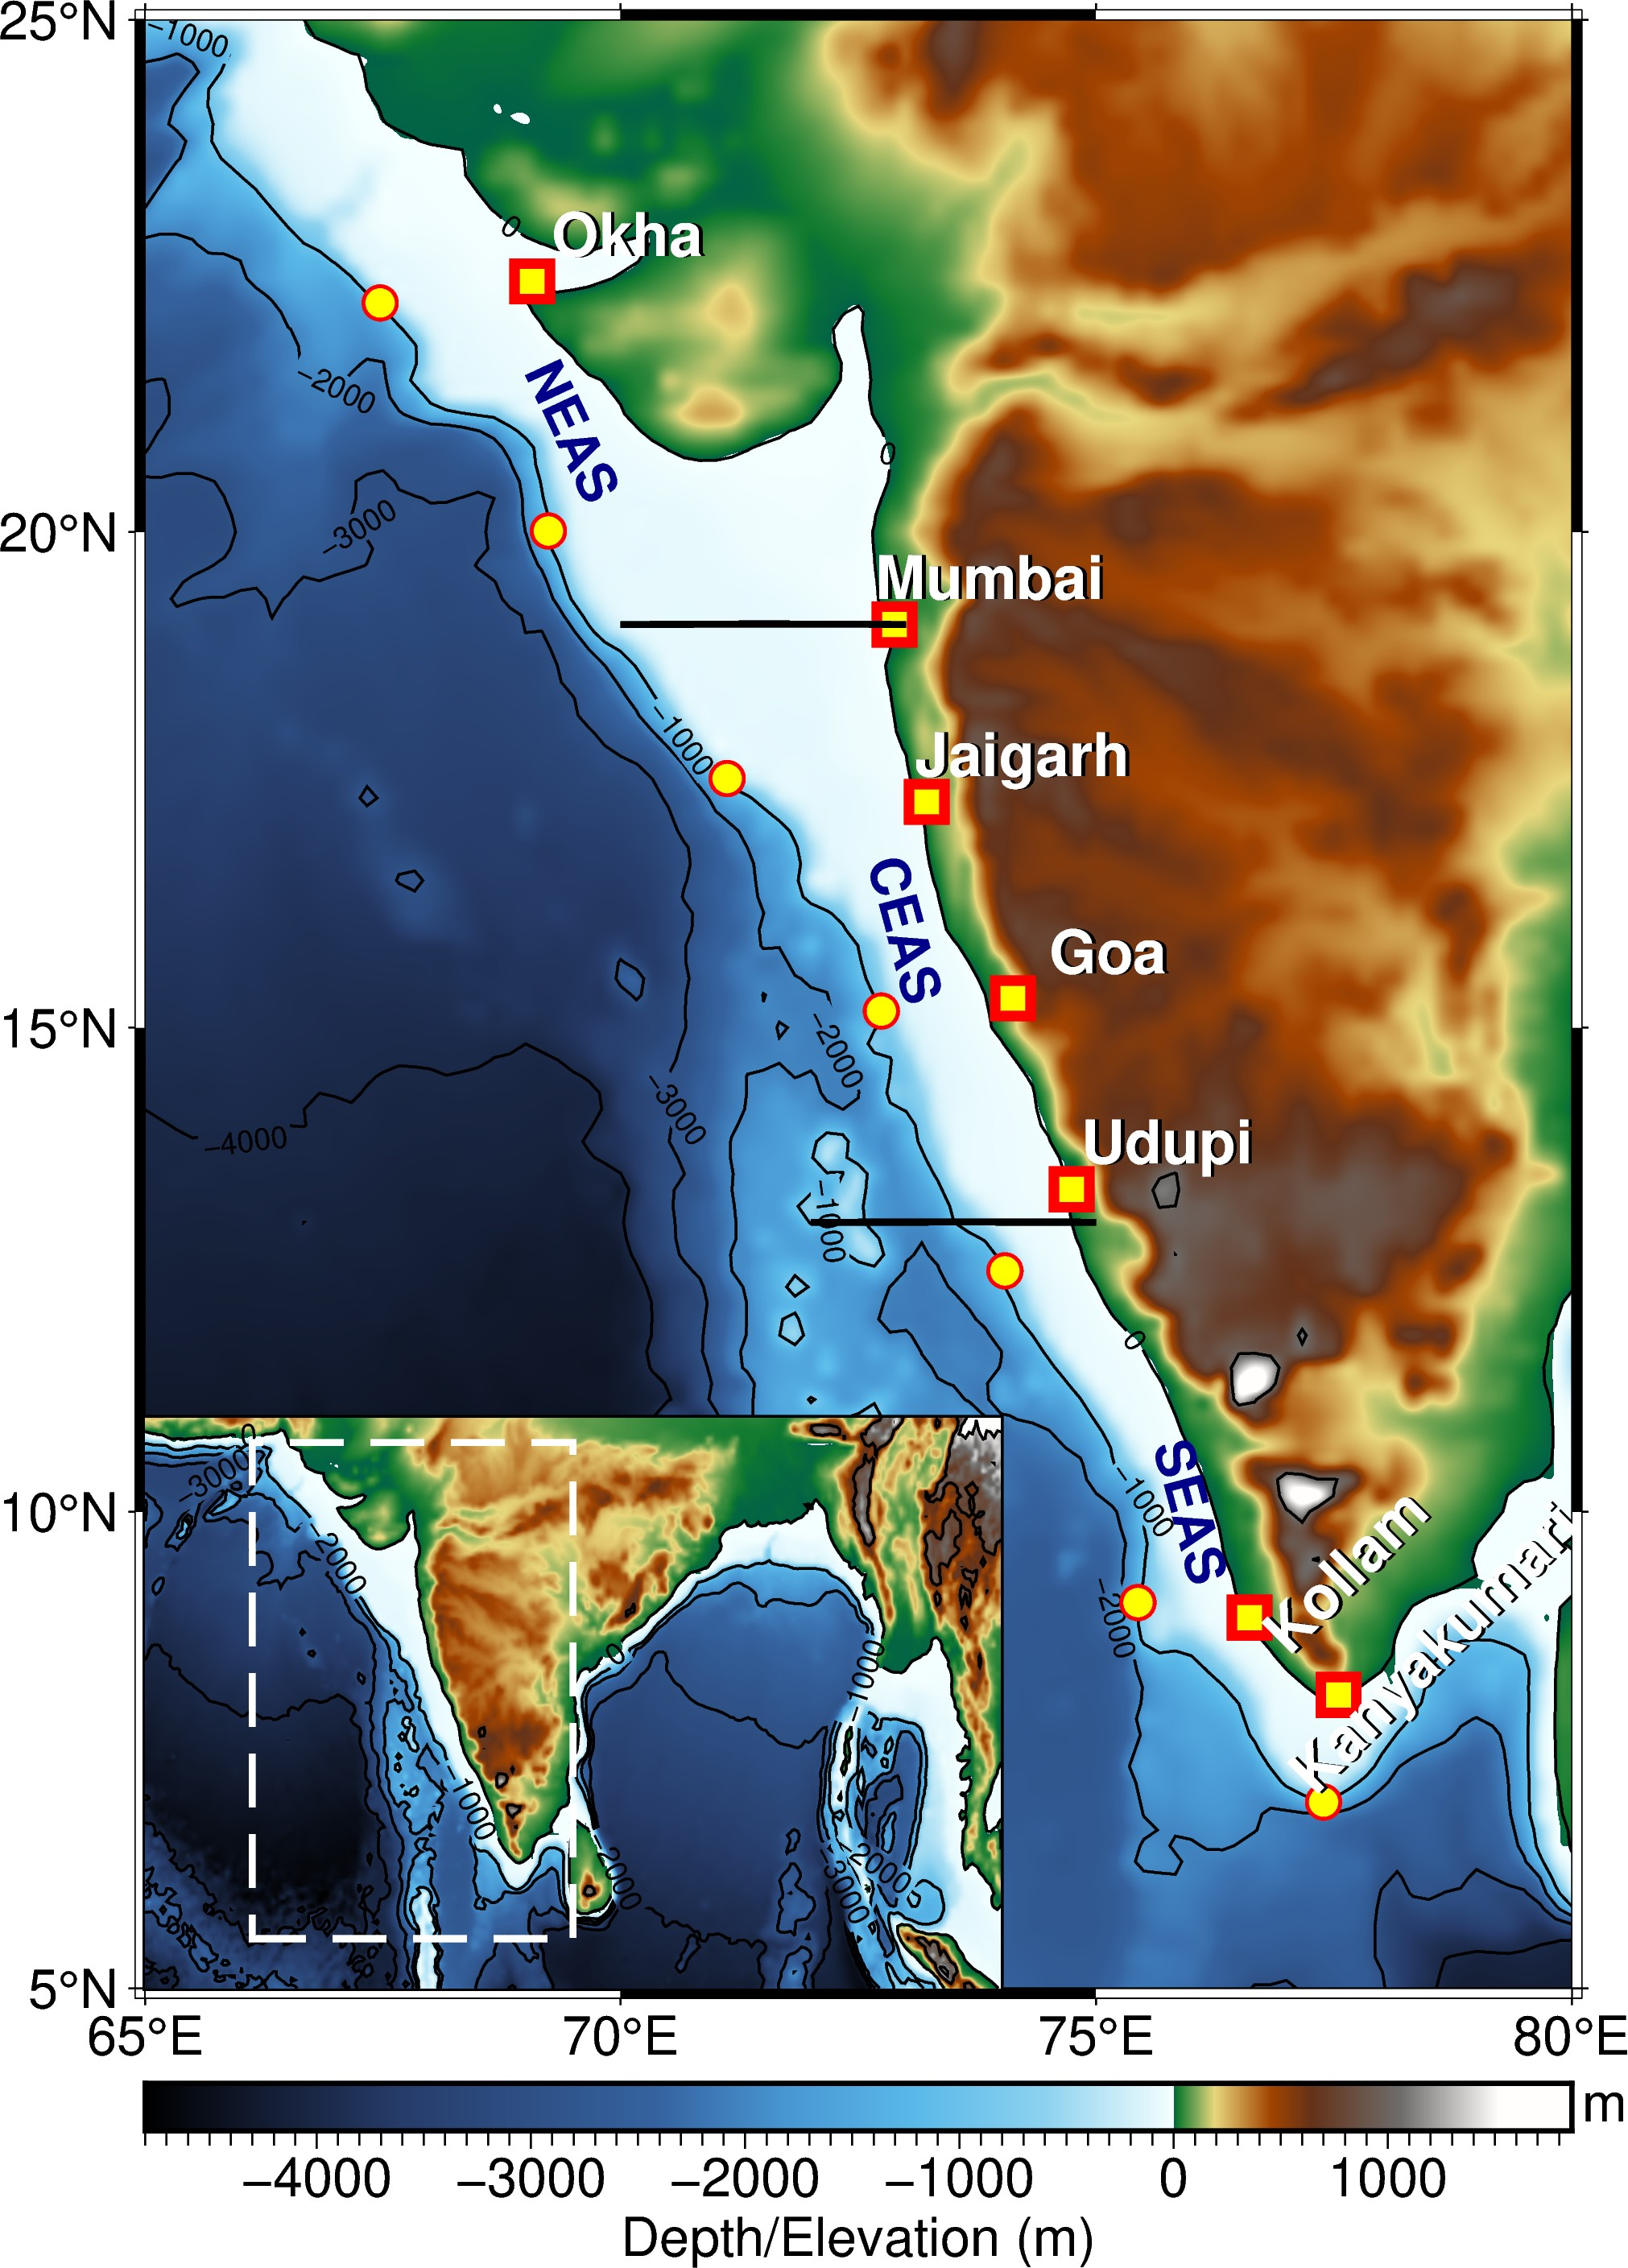
\includegraphics[width=0.6\textwidth]{/media/scilab/disk_ranjan/works/backscatter_wc/figures/adcp_moorings_new1.jpg} 
	\captionsetup{justification=justified,font=footnotesize,skip=0.05\baselineskip,width=0.8\textwidth}
	\caption{Map showing region of interest in eastern Arabian Sea. The slope moorings are
		deployed at $\sim$1000 m depth as shown in the bathymetry contour. Note the increase in shelf width as we go poleward along the coast. The mooring sites off Okha and Mumbai are in Northern EAS; Jaigarh and Goa in Central EAS while Kollam and Kanyakumari are at Southern EAS. Udupi is situated at the transition zone of Central and Southern EAS.}
	\label{fig:map}
\end{figure}

\newpage
\begin{figure}[htbp]
	\centering
	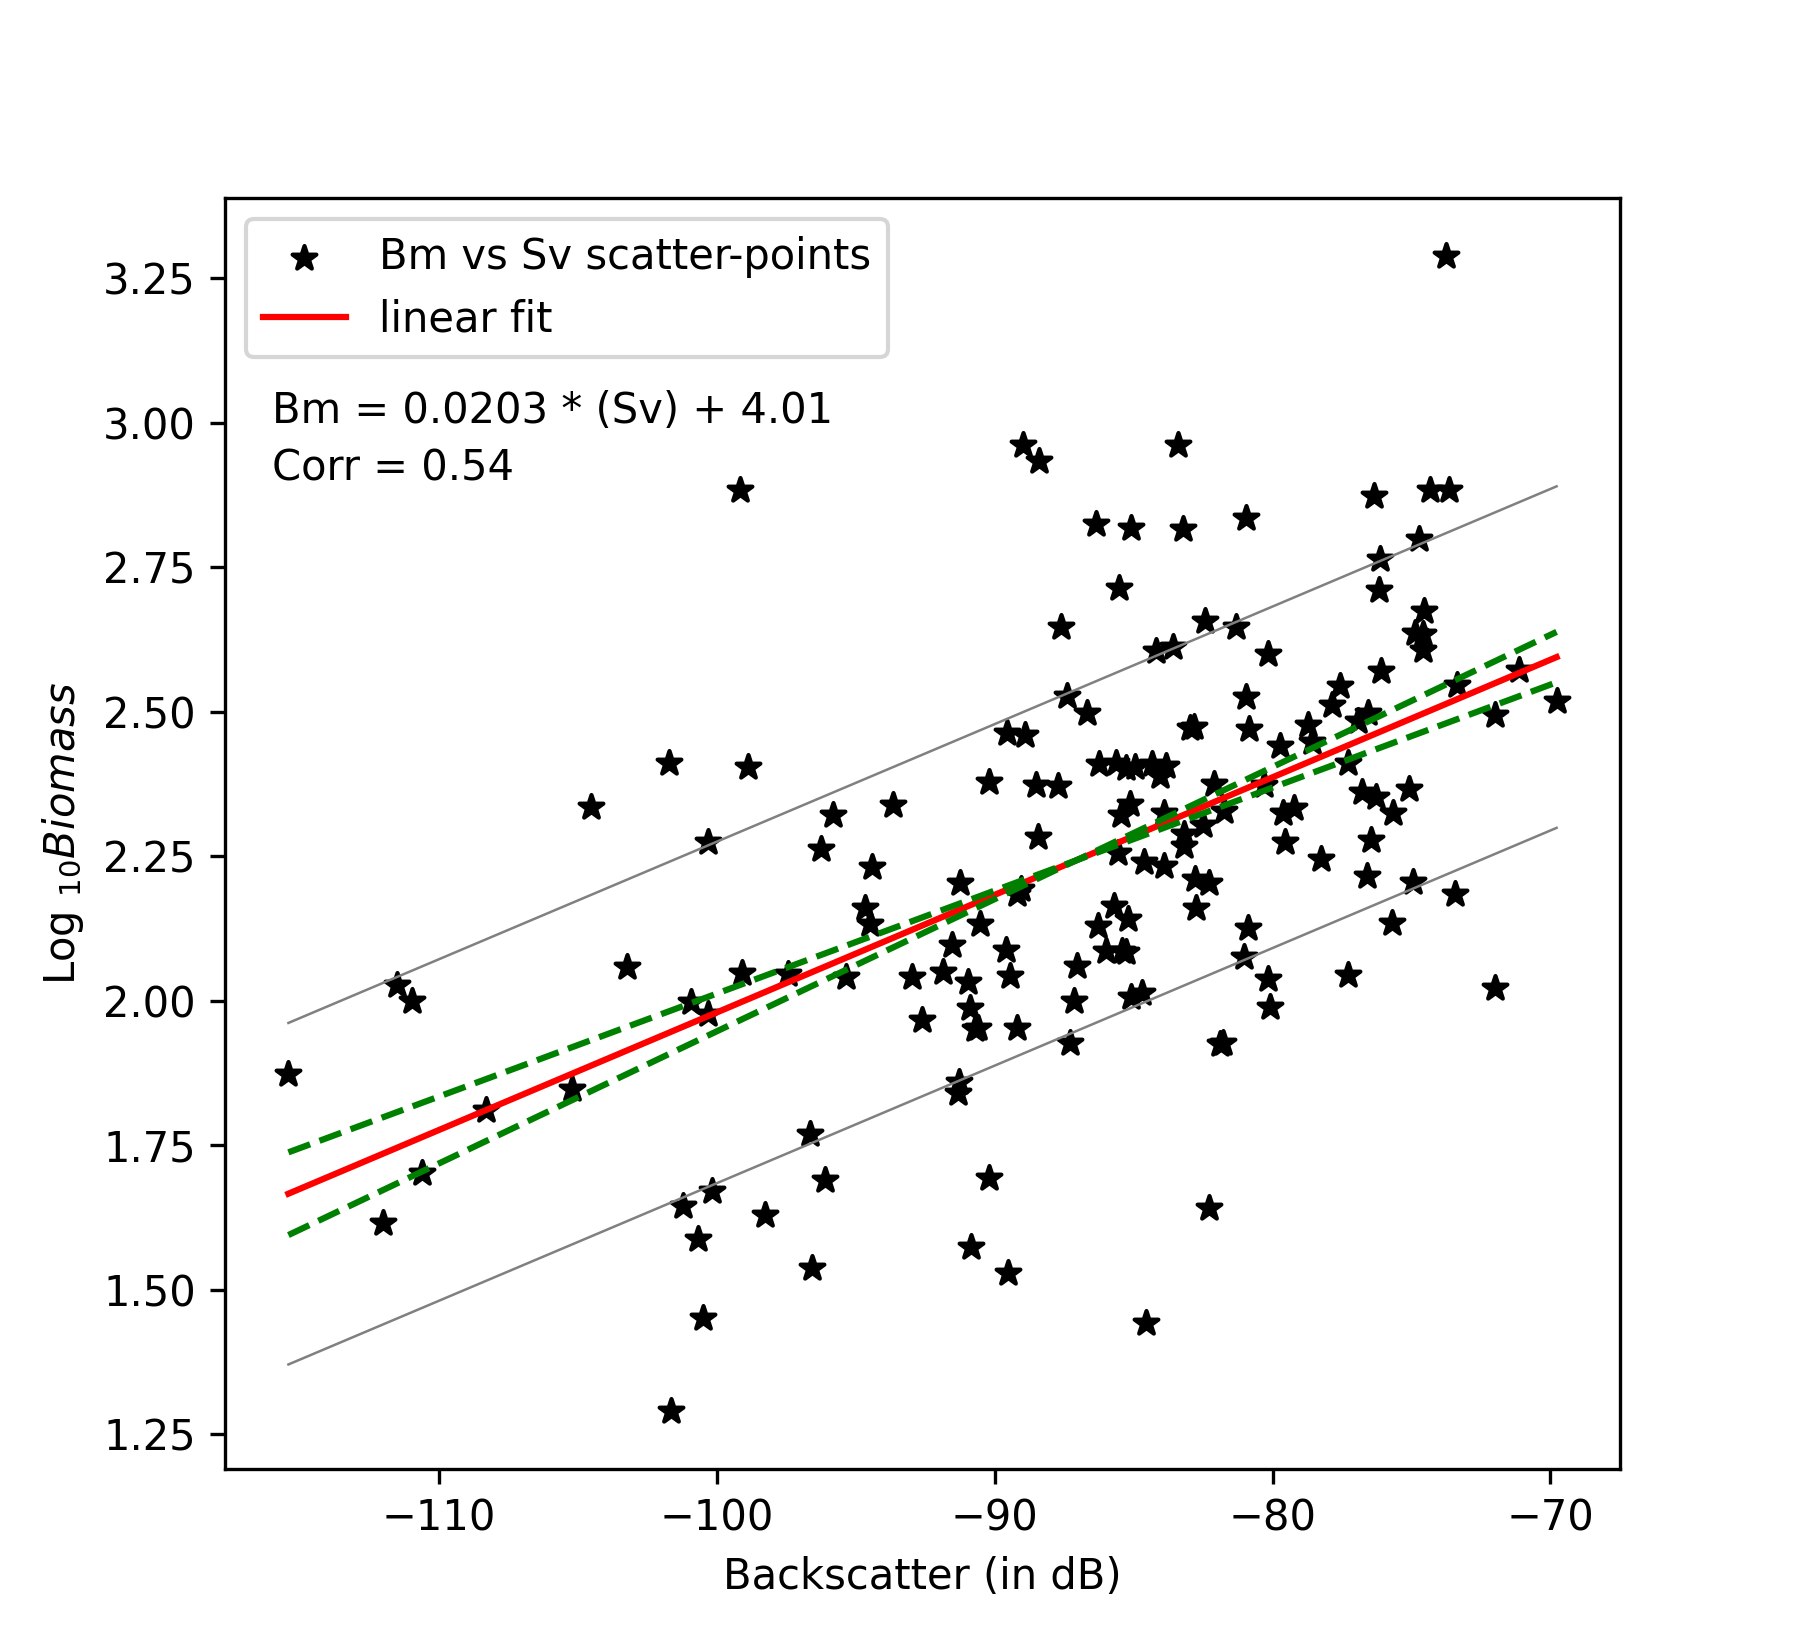
\includegraphics[width=0.5\textwidth]{/media/scilab/disk_ranjan/works/backscatter_wc/figures/backscatter_vs_biomass.png} 
	\captionsetup{justification=justified,font=footnotesize,skip=0.05\baselineskip,width=0.8\textwidth}
	\caption{The linear fit line of Biomass (log$_{10}$ scale) and backscattering strength (in dB). The linear fit line is within the error range of previous result of \citep{aparna2022seasonal} (contained 67 data points) onto which latest zooplankton volumetric sample data (159 data points) is appended. The regression equation is $y\ = (0.02 \pm\ 0.0025) \ x + (4.0144 \pm \ 0.2198) $ and correlation value of 0.54. The dashed green lines denote error range of plausible slope and intercept. From the linear equation, the upper and lower bound of error limit leads to an error bar of $\sim$14  mg~m$^{-3}$. Standard deviation $\sigma$ of log$_{10}$(Biomass) is $\pm$ 0.49, which results in the backscatter range of 48.58 dB encompassing the entire backscatter range. It signifies the robustness of zooplankton biomass dependency on ADCP measured backscattering strength.}
	\label{fig:bstobm}
\end{figure}

\newpage

\begin{figure}[htbp]
	\centering
	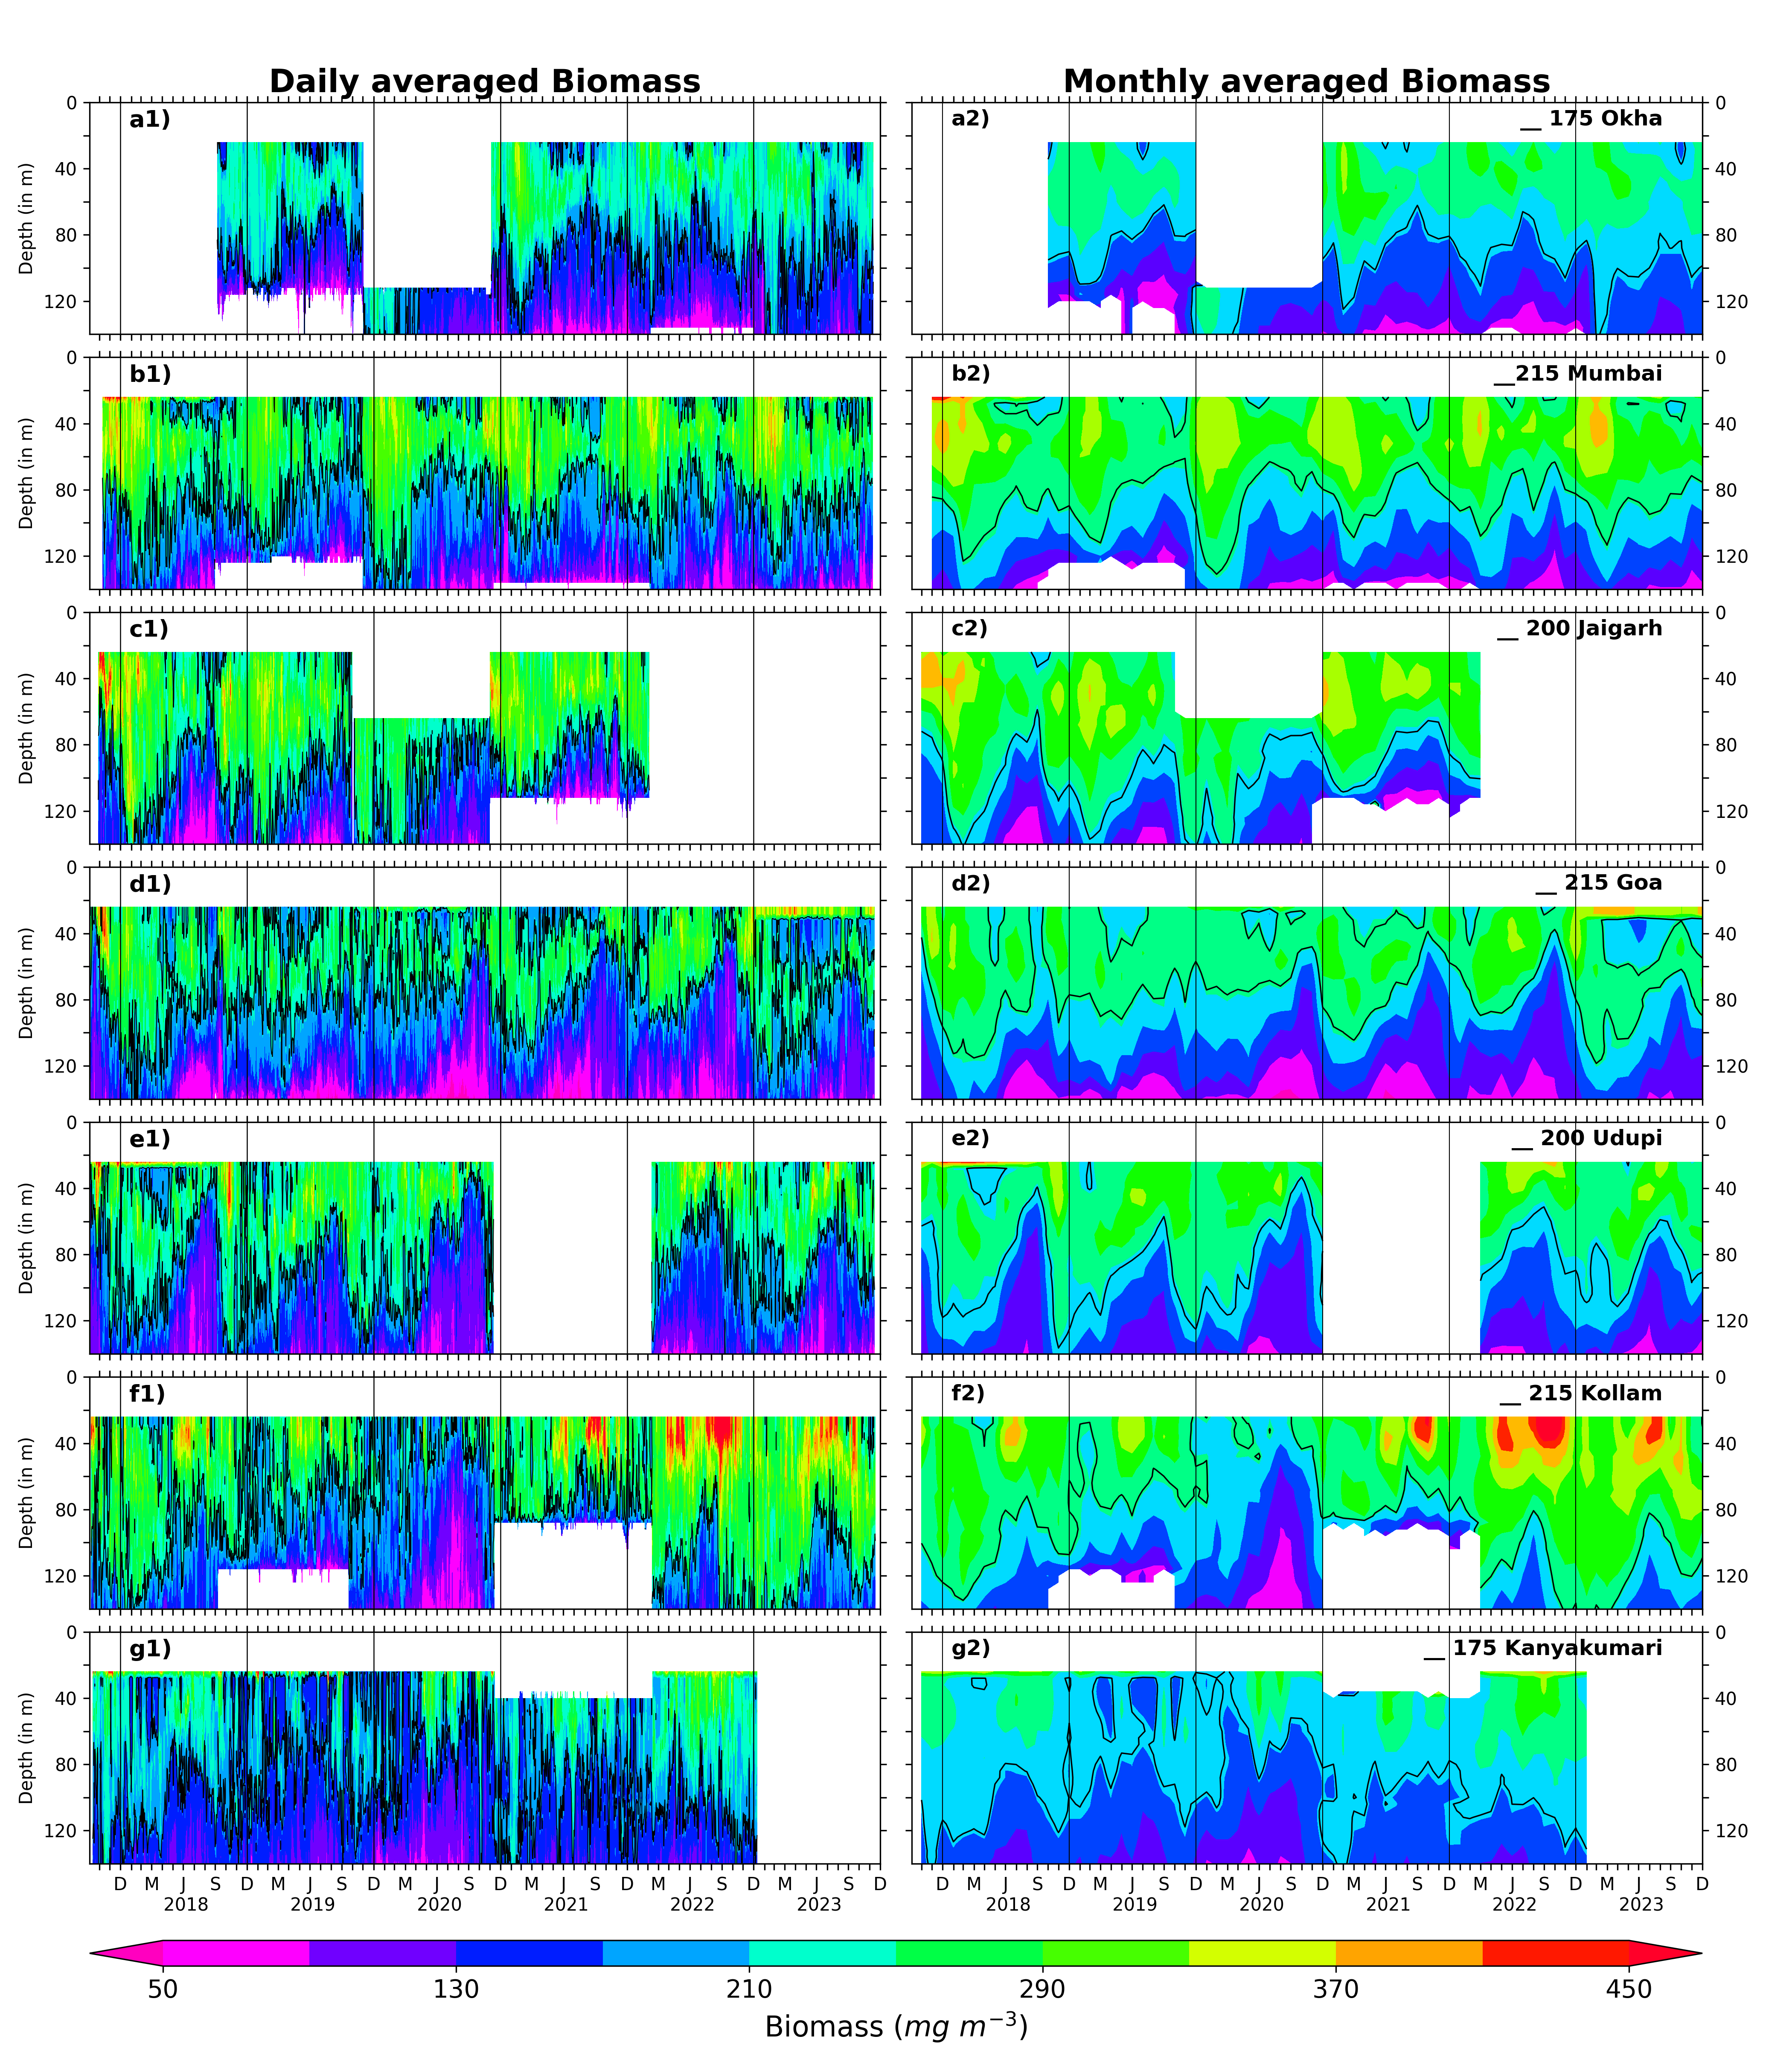
\includegraphics[width=\textwidth]{/media/scilab/disk_ranjan/works/backscatter_wc/figures/biomass_daily_monthly.png} 
	\captionsetup{justification=justified,font=footnotesize,skip=0.05\baselineskip,width=\textwidth}
	\caption{The Daily and monthly averaged biomass for EAS moorings, north (top) to south (bottom). The black contours are marking of 175 mg~m$^{-3}$ biomass for Okha and Kanyakumari; 215 mg~m$^{-3}$  for Mumbai, Goa and Kollam. The biomass contours are distinct and different based on the physico-chemical parameters and the one that best explains seasonality at respective location.  The top 10\% of data is discarded due to echo noise. The dashed line at 22 m marks the top-depth of first bin i.e, 24 m. During 2020 off Kollam, a lack of suitable biomass contour showing seasonality is due to strong interannual variations.}
	\label{fig:dailynmonthly}
\end{figure}

\begin{figure}[htbp]
	\centering
	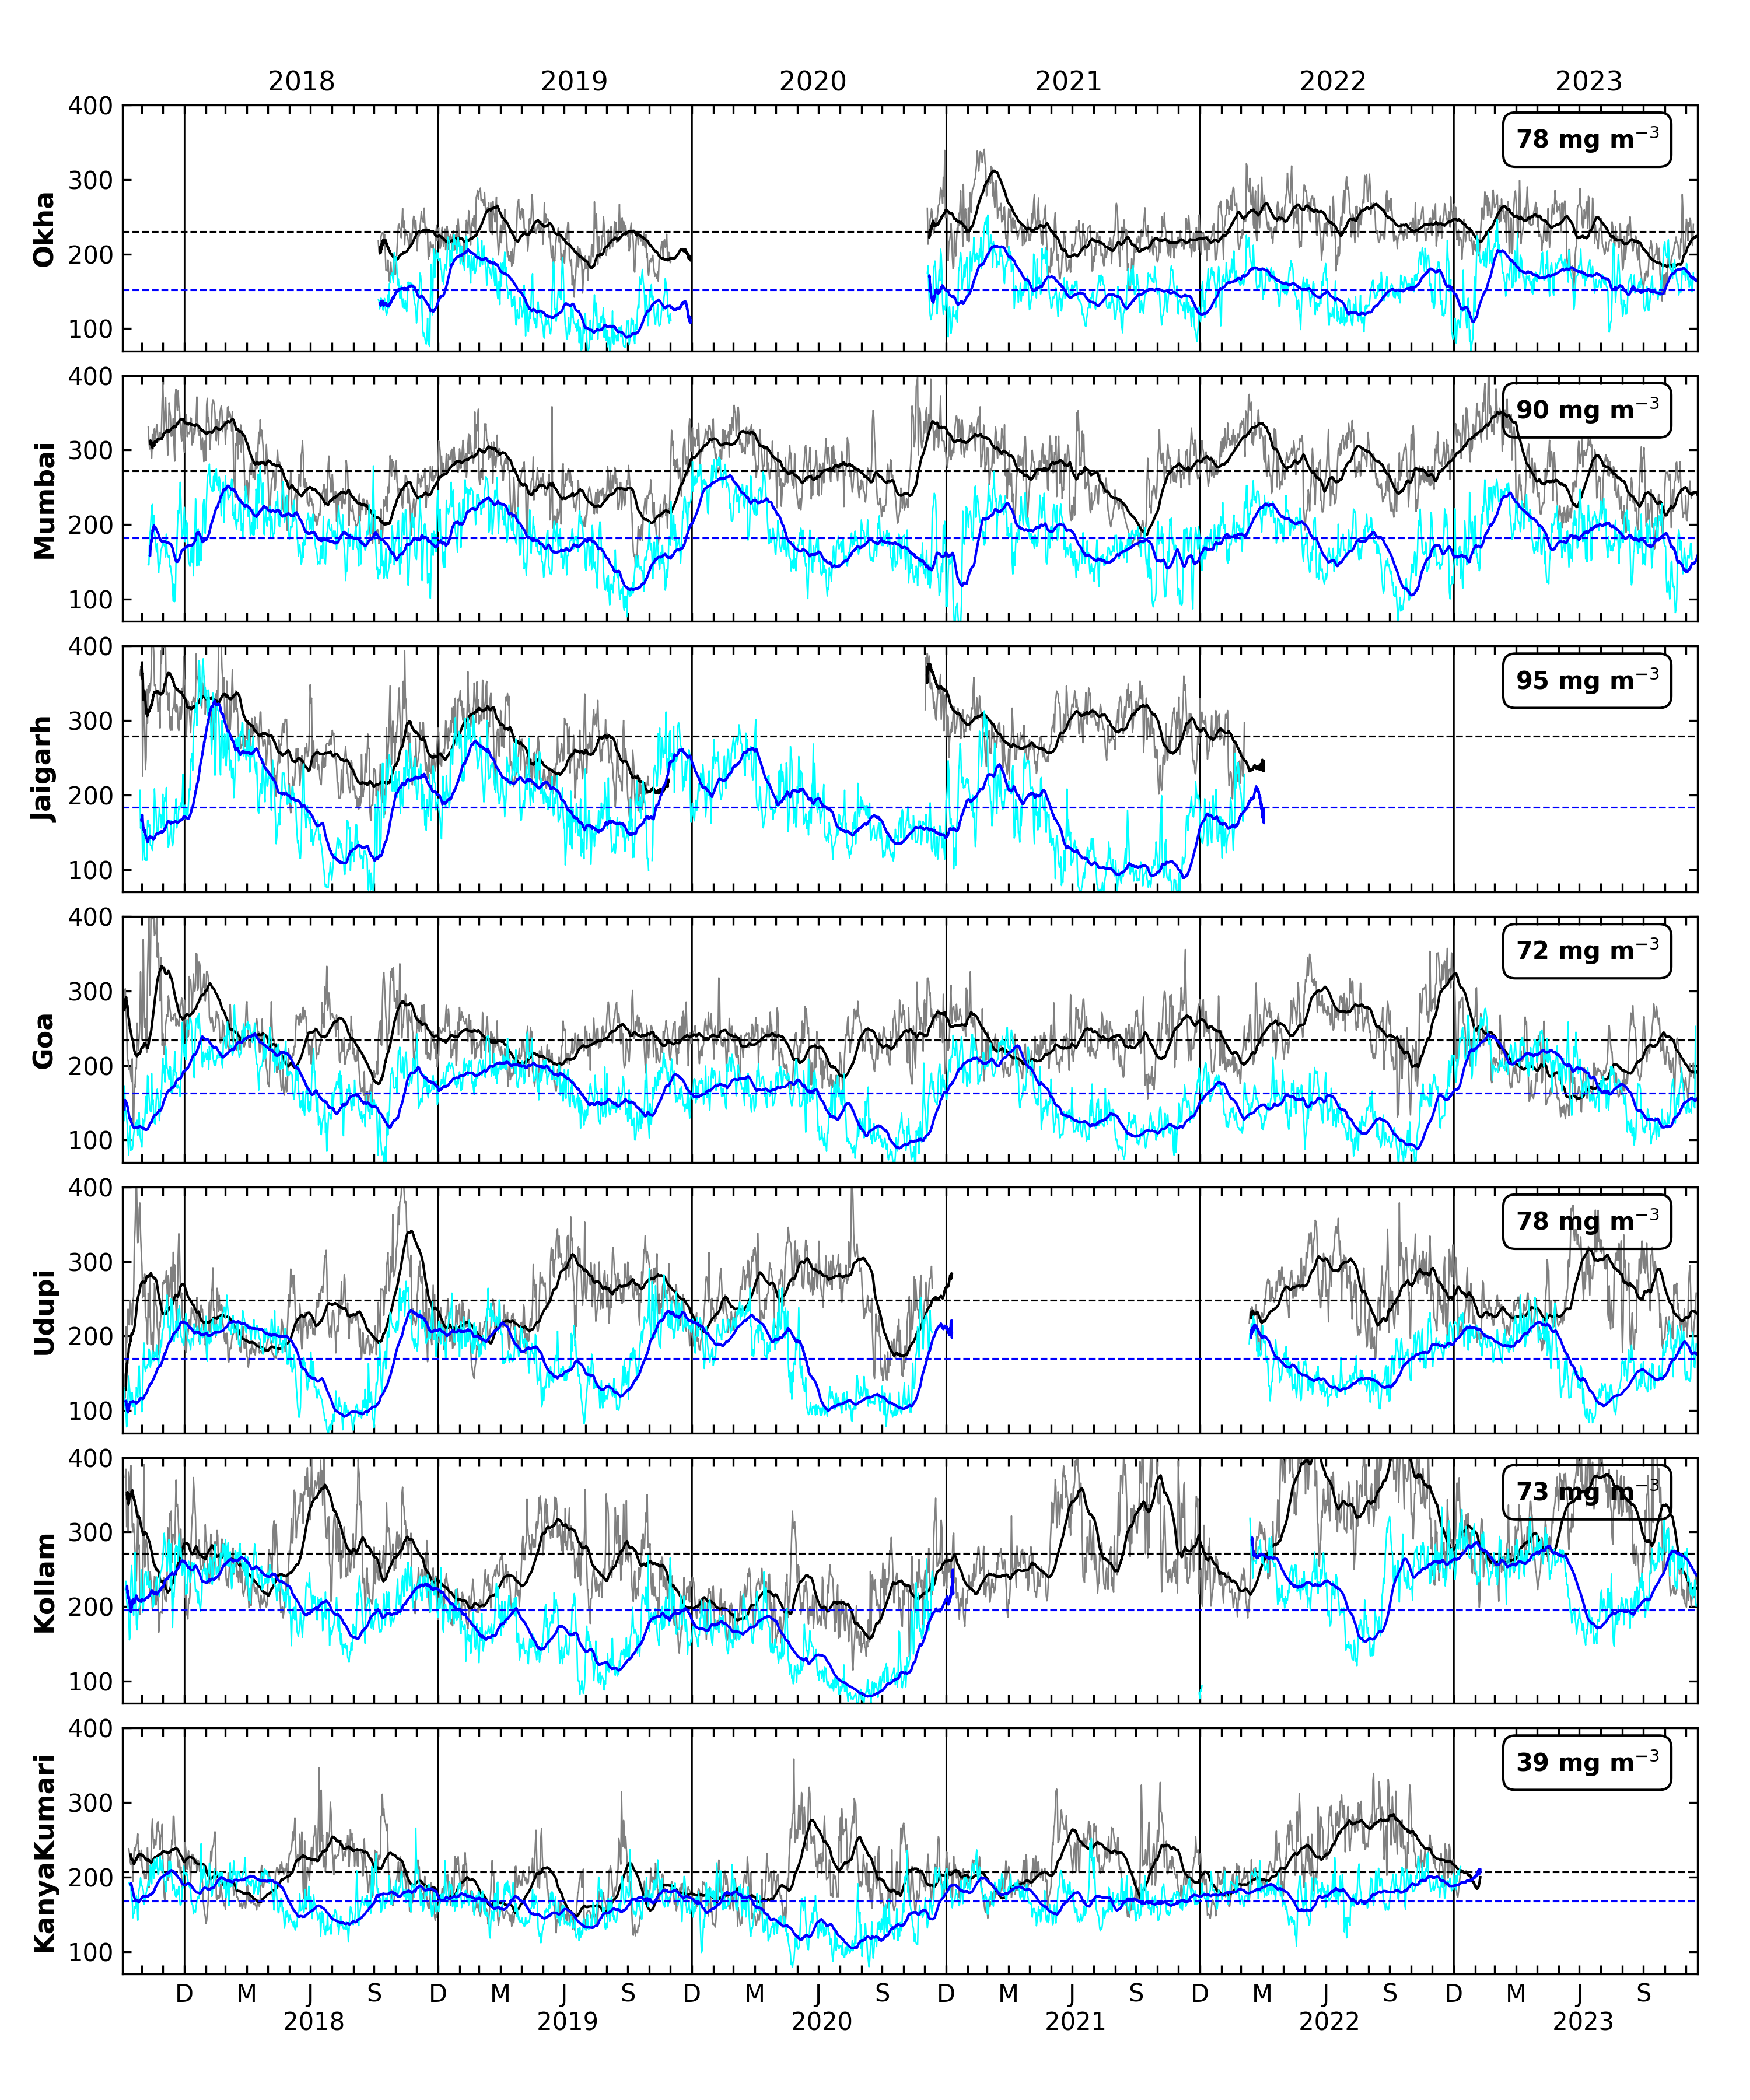
\includegraphics[width=\textwidth]{/media/scilab/disk_ranjan/works/backscatter_wc/figures/biomass_40m_104m.png} 
	\captionsetup{justification=justified,font=footnotesize,skip=0.05\baselineskip,width=\textwidth}
	\caption{The biomass at depth of 40 m (grey, black) and 104 m (cyan, blue) and ZSS (pink, red), the lighter (darker) shades shows daily (30 day rolling averaged) sample, respectively. The mean biomass at 40 and 104 and mean ZSS is shown in top right corresponding to black, blue and red. Notice the spikes (bursts) seen in the daily (rolling mean) data of biomass at 40 m that lasts few days (few days to weeks), e.g., during many isolated days of June of 2020 (during entire June--July of 2020). These spikes and bursts are seen at all locations and both at 40 and 104 m, albeit with a varied magnitude.}
	\label{fig:compfourty}
\end{figure}


\begin{figure}[htbp]
	\centering
	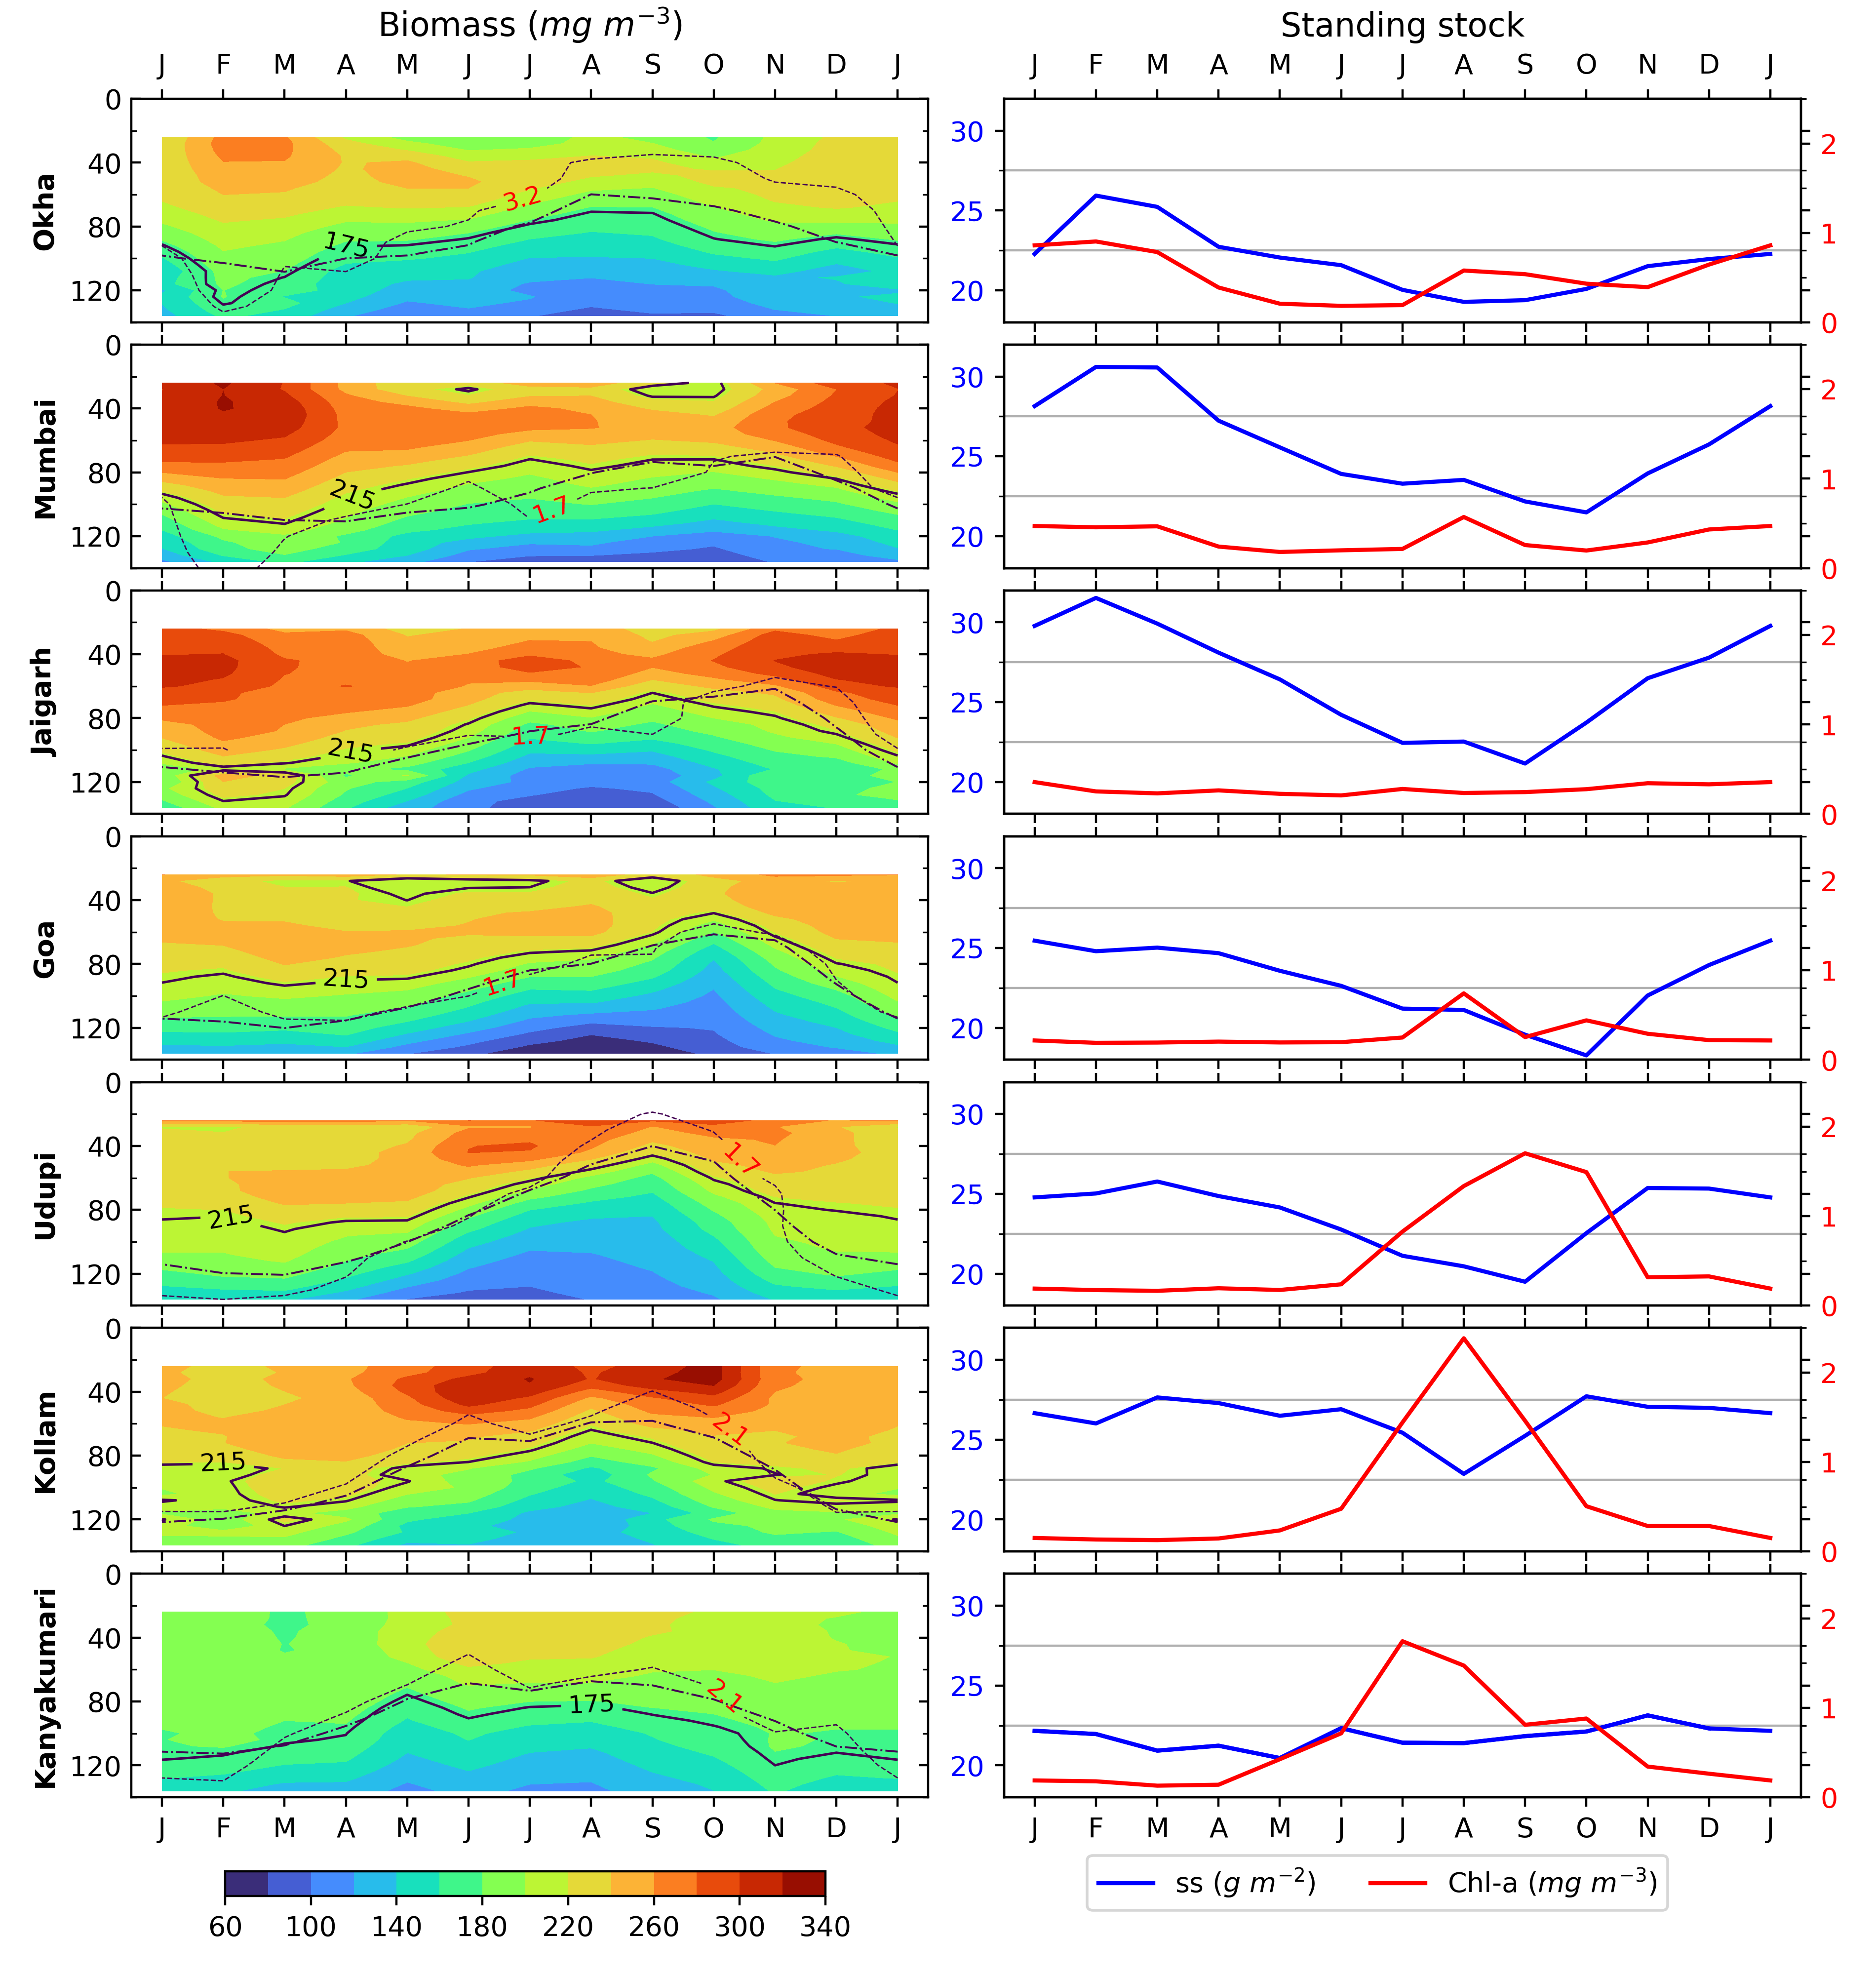
\includegraphics[width=\textwidth]{/media/scilab/disk_ranjan/works/backscatter_wc/figures/climatology_biomass_ss_chl.png} 
	\captionsetup{justification=justified,font=footnotesize,skip=0.05\baselineskip,width=\textwidth}
	\caption{Monthly climatology of zooplankton biomass is shown in left panels for 7 locations, (top to bottom is southward). The D175 and D215 are shown in solid lines; dashed line represents the depth of 23 C isotherm; oxygen contours are shown in dotted lines and labeled for each mooring. The right set of panel plots is showing ZSS (24--140 biomass integral) and chl-a climatology for corresponding locations.}
	\label{fig:zsschlclim}
\end{figure}



\begin{figure}[htbp]
	\centering
	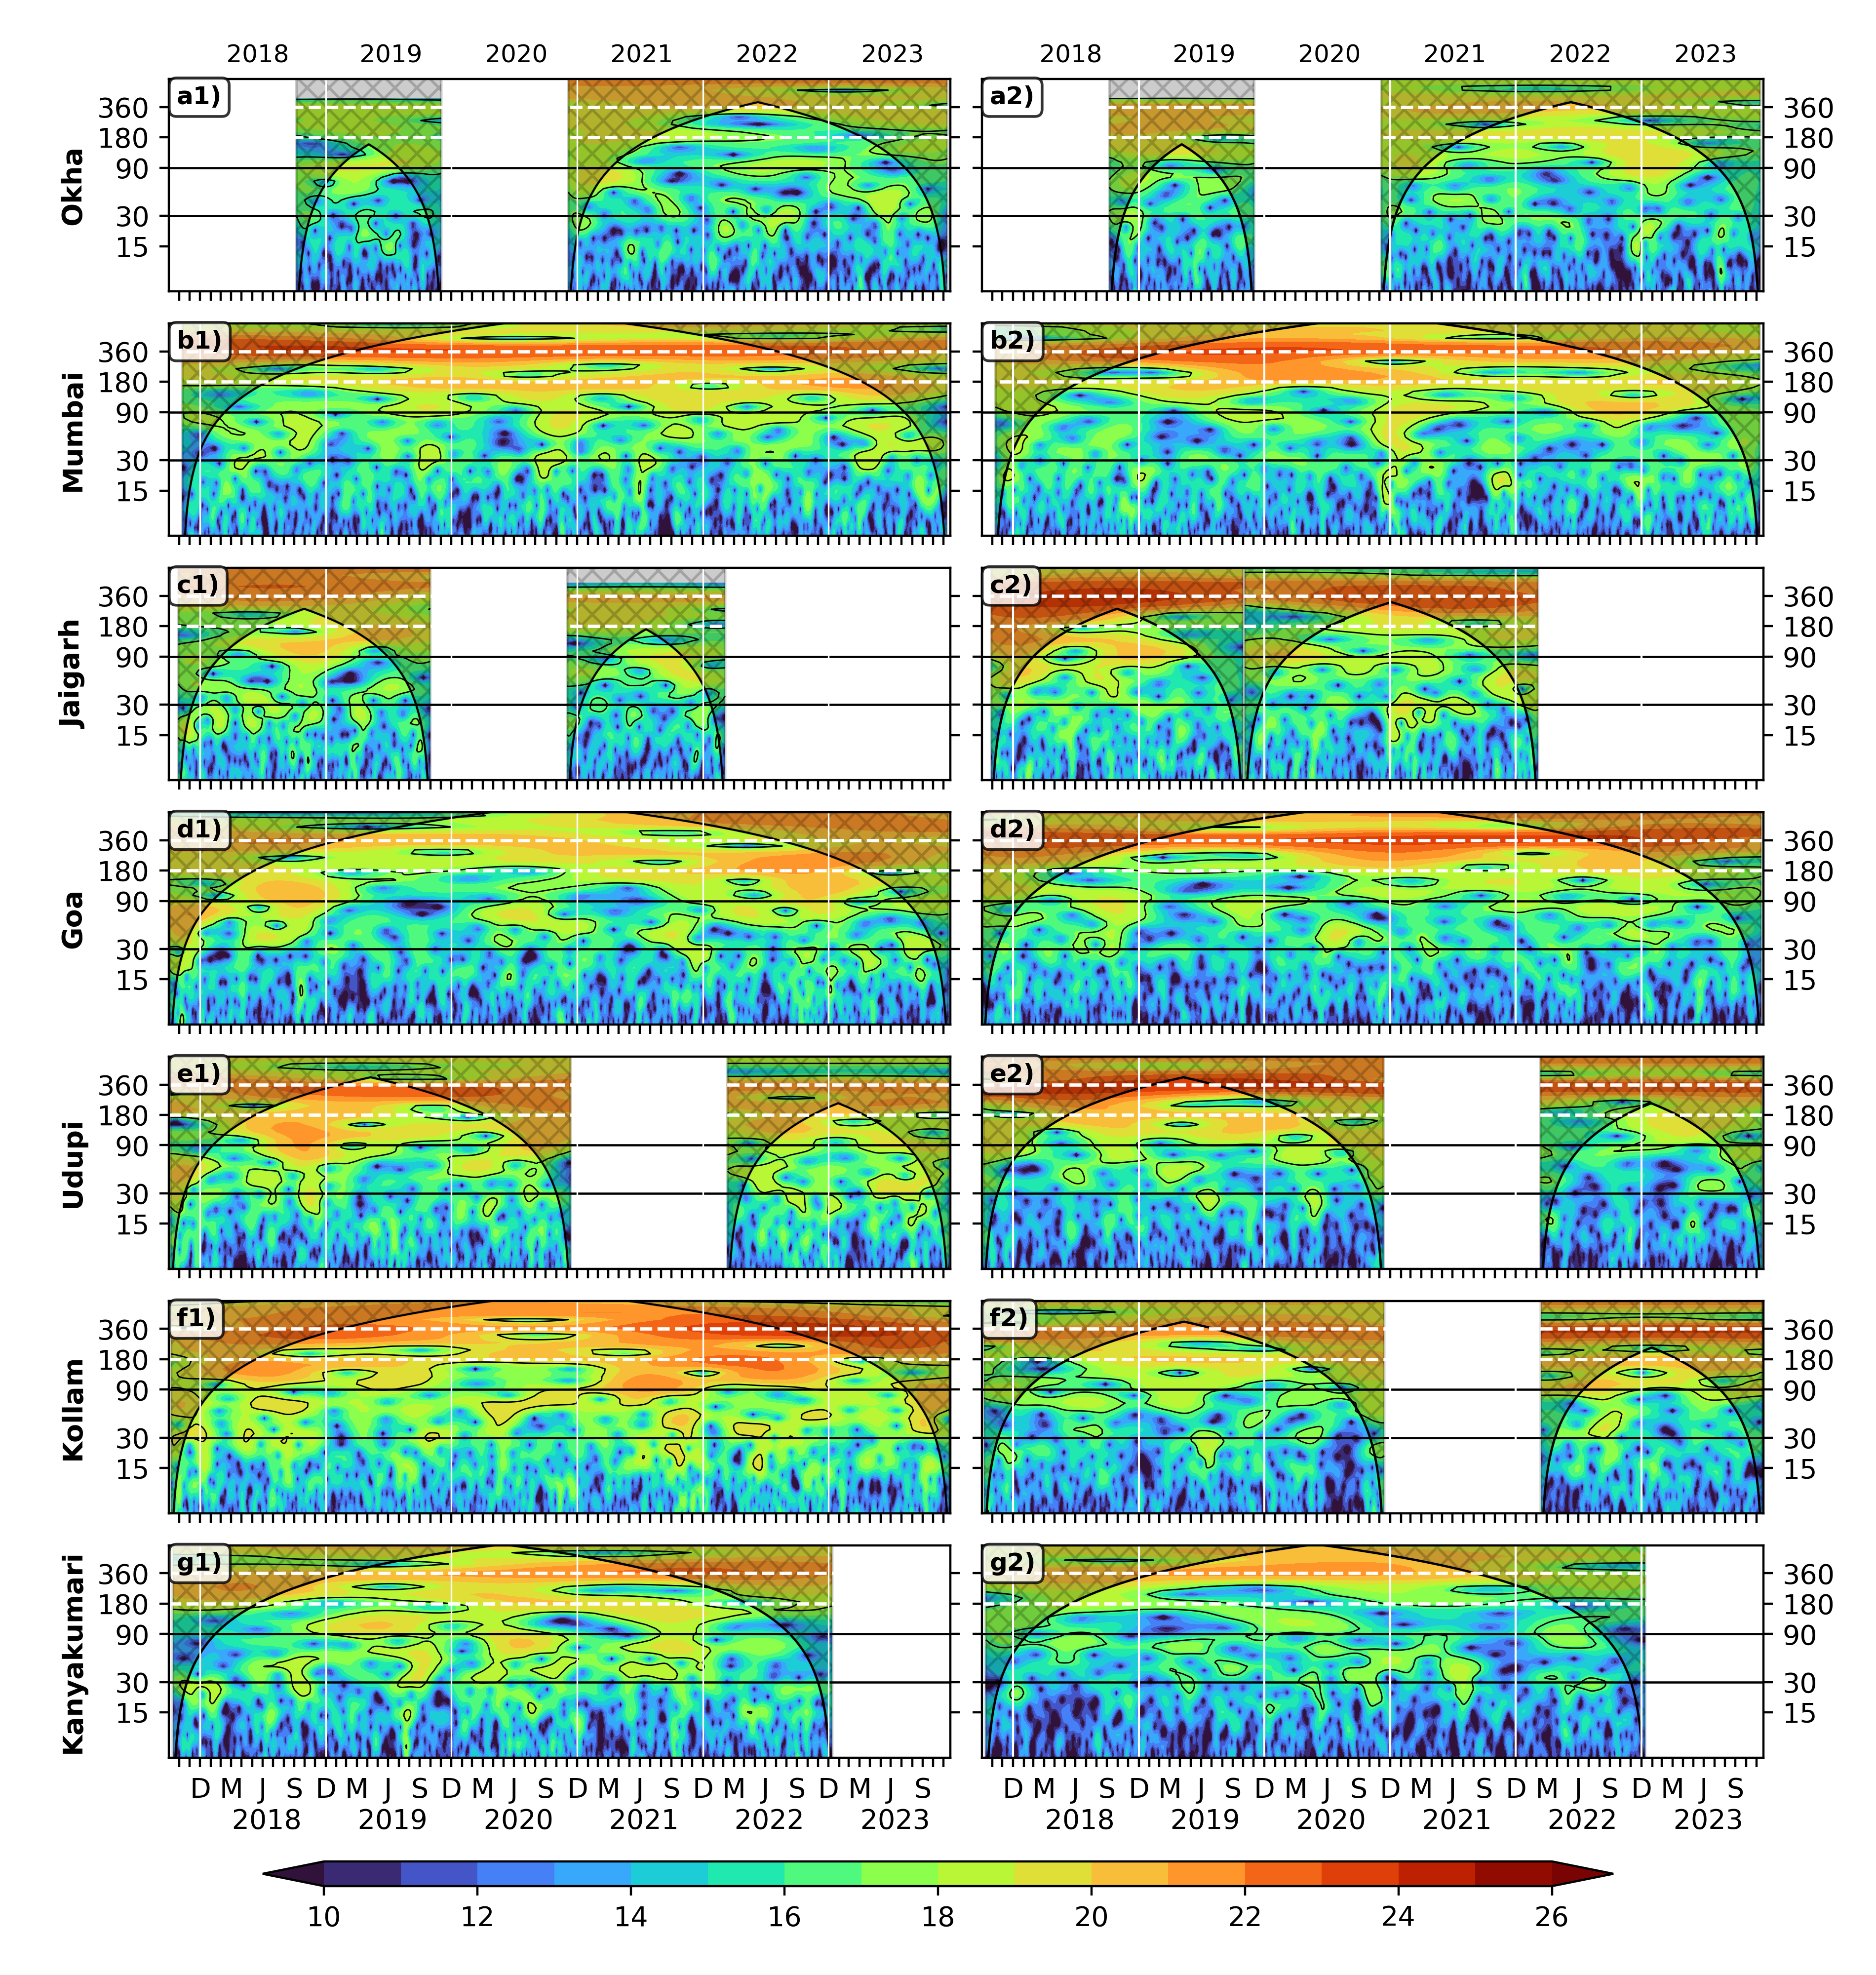
\includegraphics[width=\textwidth]{/media/scilab/disk_ranjan/works/backscatter_wc/figures/west_coast_wavelet_40m_104m.png} 
	\captionsetup{justification=justified,font=footnotesize,skip=0.05\baselineskip,width=\textwidth}
	\caption{Wavelet power spectra (Morlet) of the 40 m (left panel) and 104 m (right panel) zooplankton biomass plotted against time as abscissa and period in days as ordinate. The wavelet power is in log$_2$ scale, the 95\% significance is marked in black contours; the cross-shaded region falls under cone of influence. The horizontal dashed white (solid black) lines shows annual and semi-annual periods (intraseasonal band). Vertical white lines separates years.}
	\label{fig:wave40104}
\end{figure}


\begin{figure}[htbp]
	\centering
	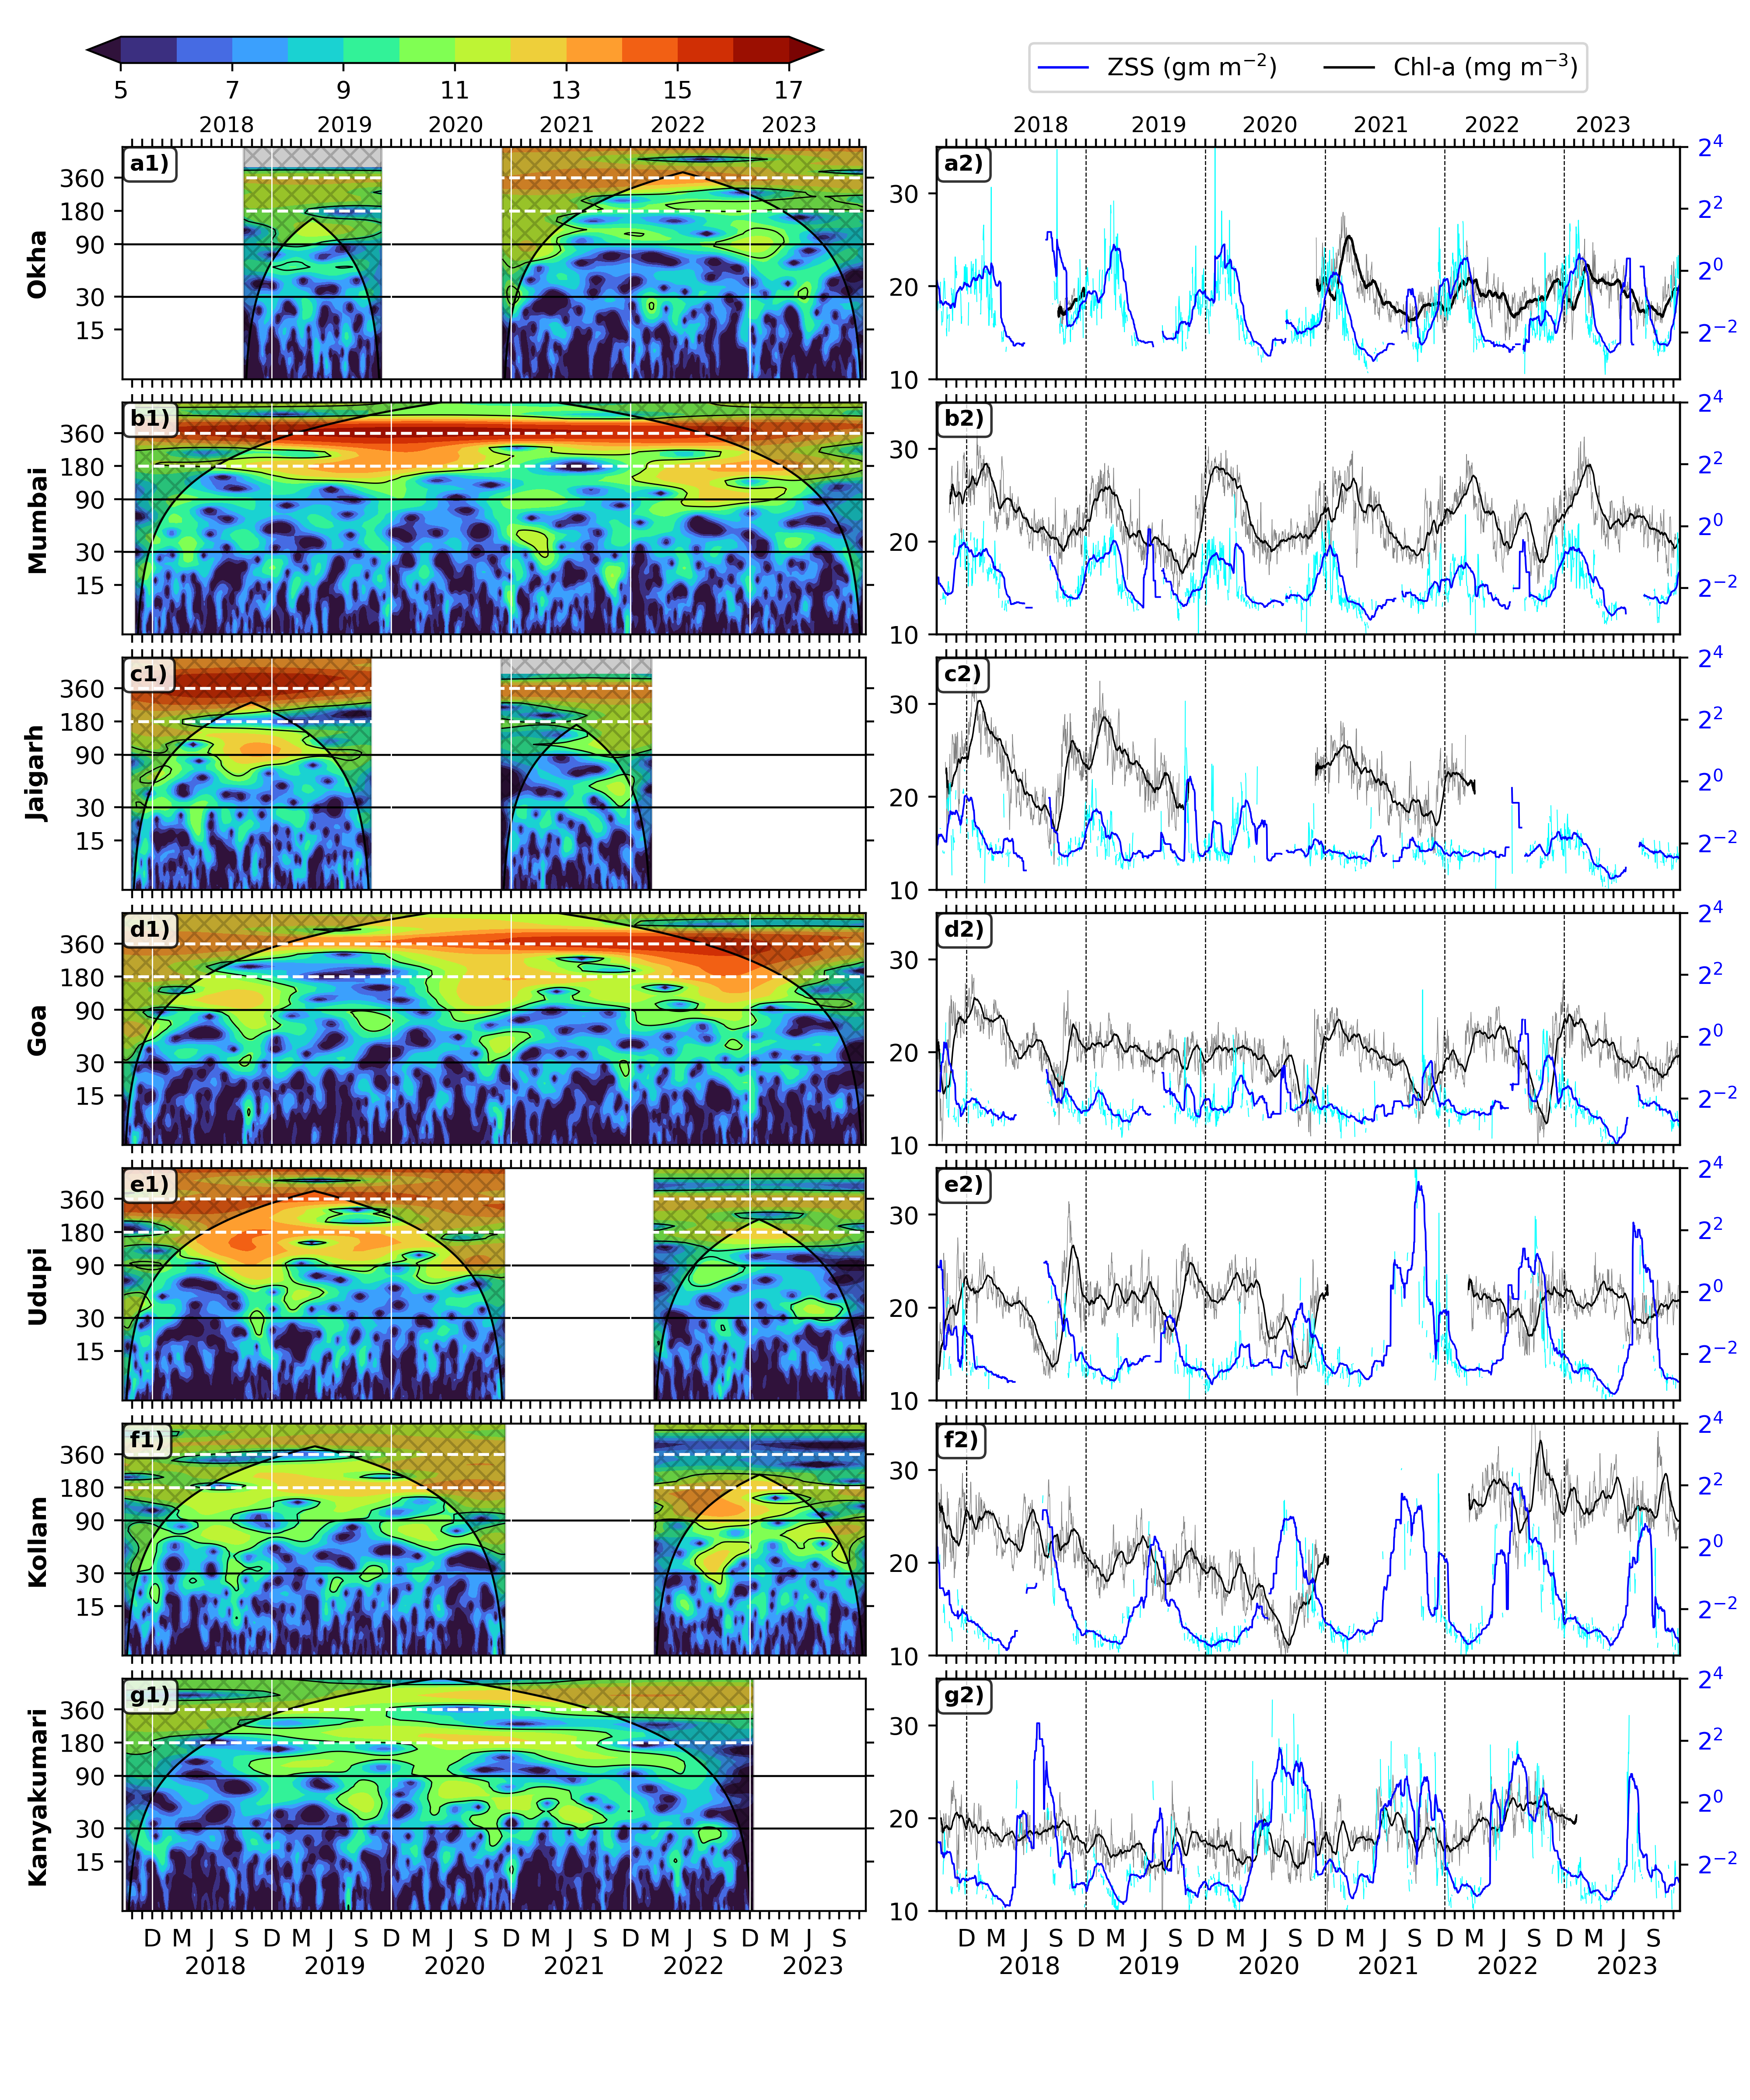
\includegraphics[width=\textwidth]{/media/scilab/disk_ranjan/works/backscatter_wc/figures/west_coast_wavelet_ss_scale.png} 
	\captionsetup{justification=justified,font=footnotesize,skip=0.05\baselineskip,width=\textwidth}
	\caption{Wavelet power spectra (Morlet) of zooplankton standing stock plotted against time as abscissa and period in days as ordinate. The wavelet power is in log$_2$ scale, the 95\% significance is marked in black contours; The vertical white lines separates years. The right side panel shows the ZSS (24--120 m biomass integral) time series of 30 day rolling mean data (black) overlaid upon daily data (Grey). The 30 day rolling mean data of chl-a (solid blue) is plotted over its daily data (cyan).}
	\label{fig:wavess}
\end{figure}



\begin{figure}[htbp]
	\centering
	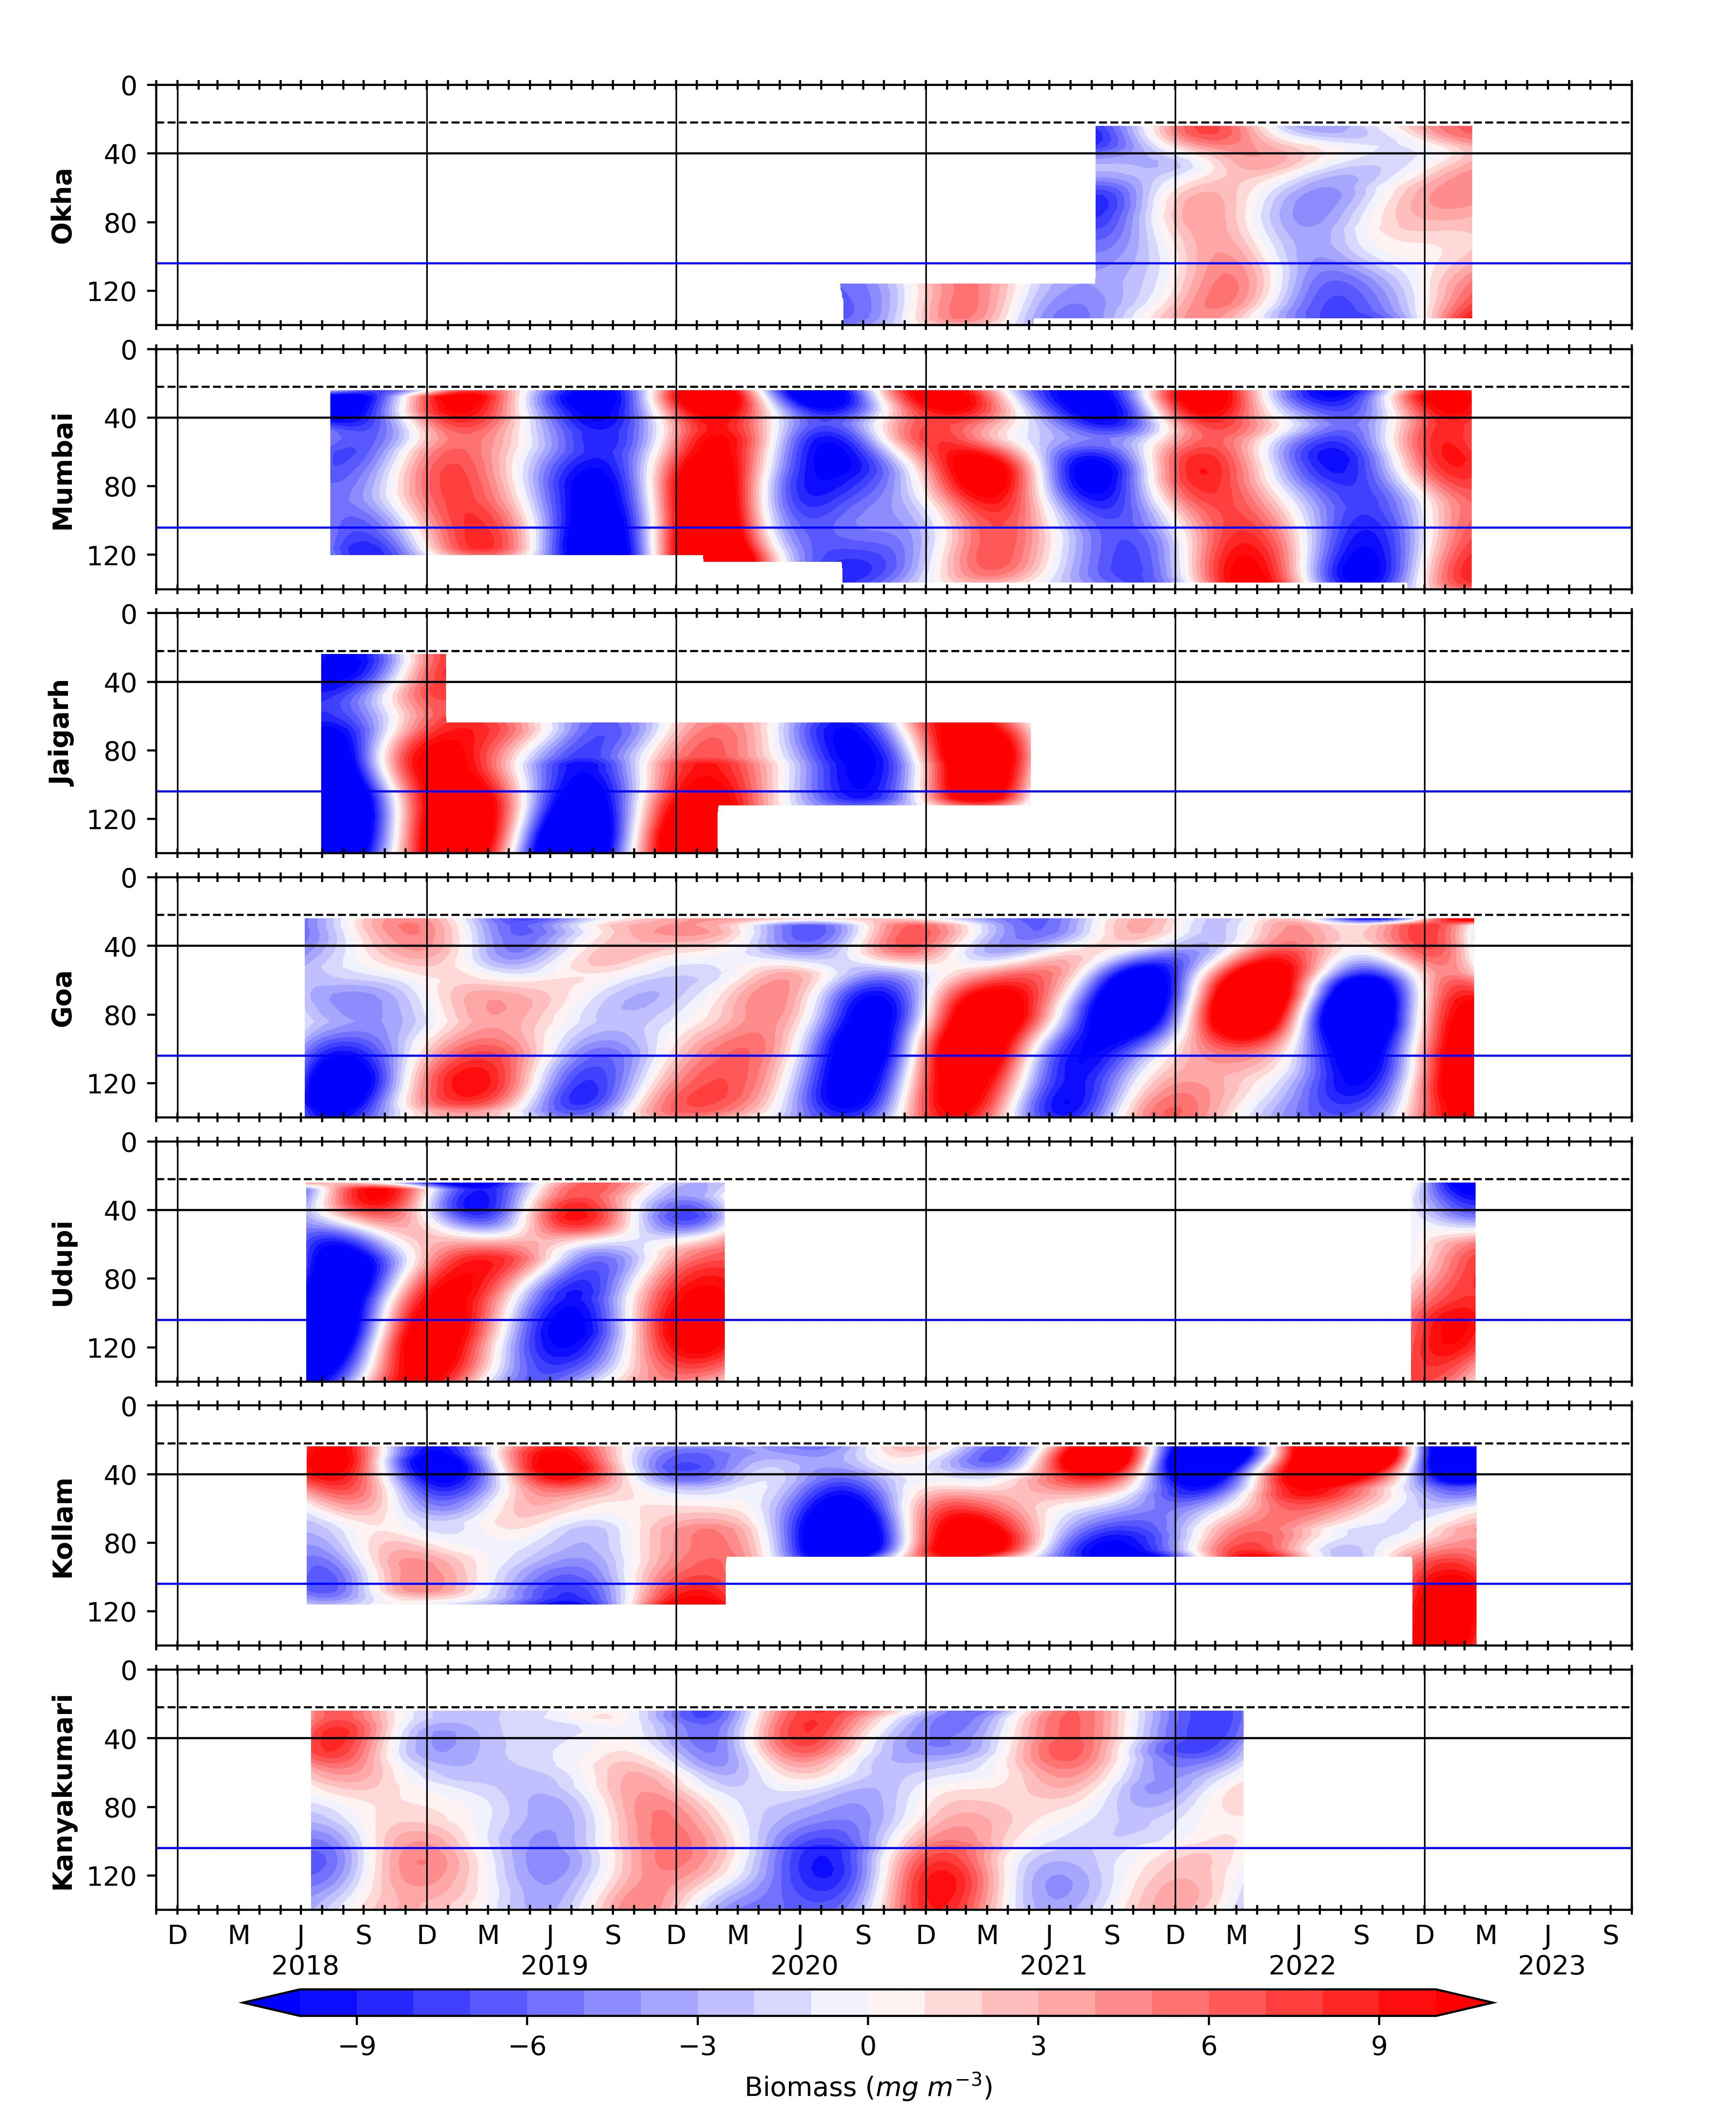
\includegraphics[width=\textwidth]{/media/scilab/disk_ranjan/works/backscatter_wc/figures/annual_300_400_451_1.jpeg} 
	\captionsetup{justification=justified,font=footnotesize,skip=0.05\baselineskip,width=\textwidth}
	\caption{The biomass variation occurring in annual band (300 to 400 days). Owing to the presence of seasonal reversal of current, there is a variation driven by associated upwelling (downwelling) processes in summer (winter) monsoon. The horizontal black and blue lines is for 40 and 104 m, and the standard deviation of biomass at those depths are shown in respective colors at top right corner of each panel; vertical black lines separate the years. The dashed line at 22 m marks the top-depth of first bin i.e, 24 m and solid magenta curves denotes D215 (D175 off Okha and Kanyakumari)}
	\label{fig:annual}
\end{figure}



\begin{figure}[htbp]
	\centering
	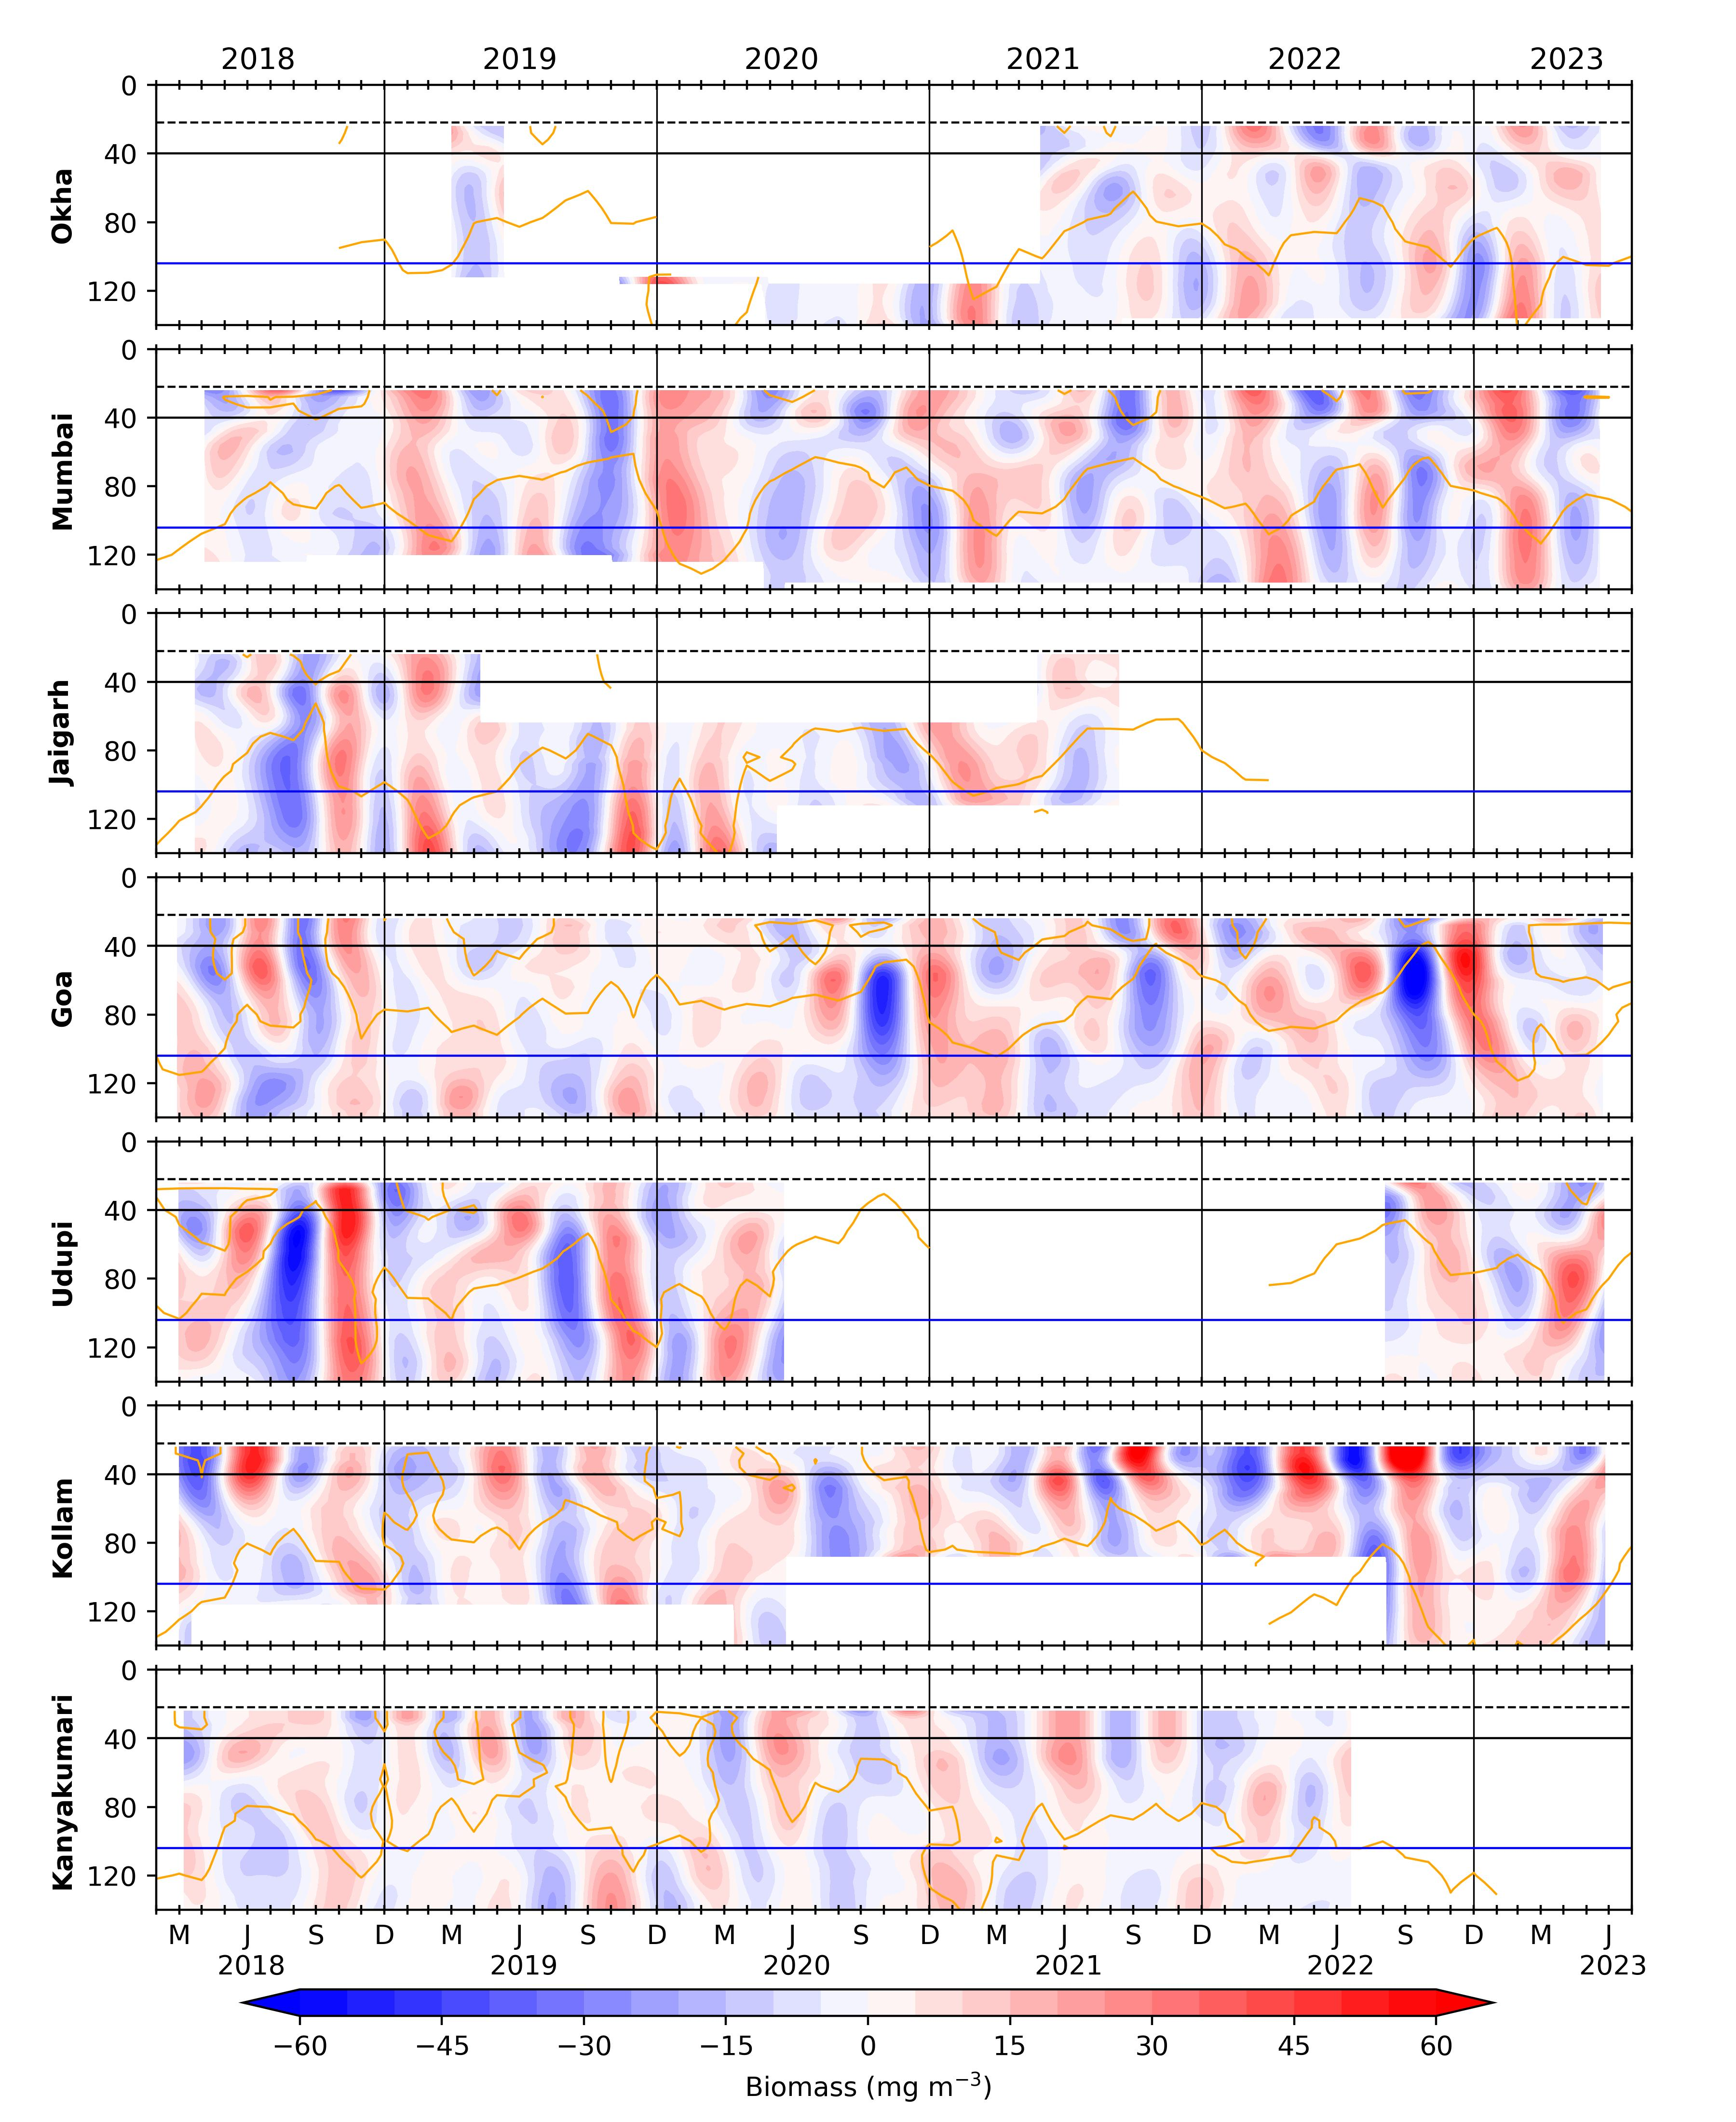
\includegraphics[width=\textwidth]{/media/scilab/disk_ranjan/works/backscatter_wc/figures/intraannual_100_250_351.jpeg} 
	\captionsetup{justification=justified,font=footnotesize,skip=0.05\baselineskip,width=\textwidth}
	\caption{The biomass variation occurring in 100 to 250 days period (between the seasons and within a year record or intra-annual band) is obtained using a band pass filter. The horizontal black and blue lines is for 40 and 104 m,
	%and the standard deviation of biomass at those depths are shown in respective colors at top right corner of each panel;
	vertical black lines separate the years. The dashed line at 22 m marks the top-depth of first bin i.e, 24 m and solid magenta curves denotes D215 (D175 off Okha and Kanyakumari). }
	\label{fig:intraannual}
\end{figure}

\begin{figure}[htbp]
	\centering
	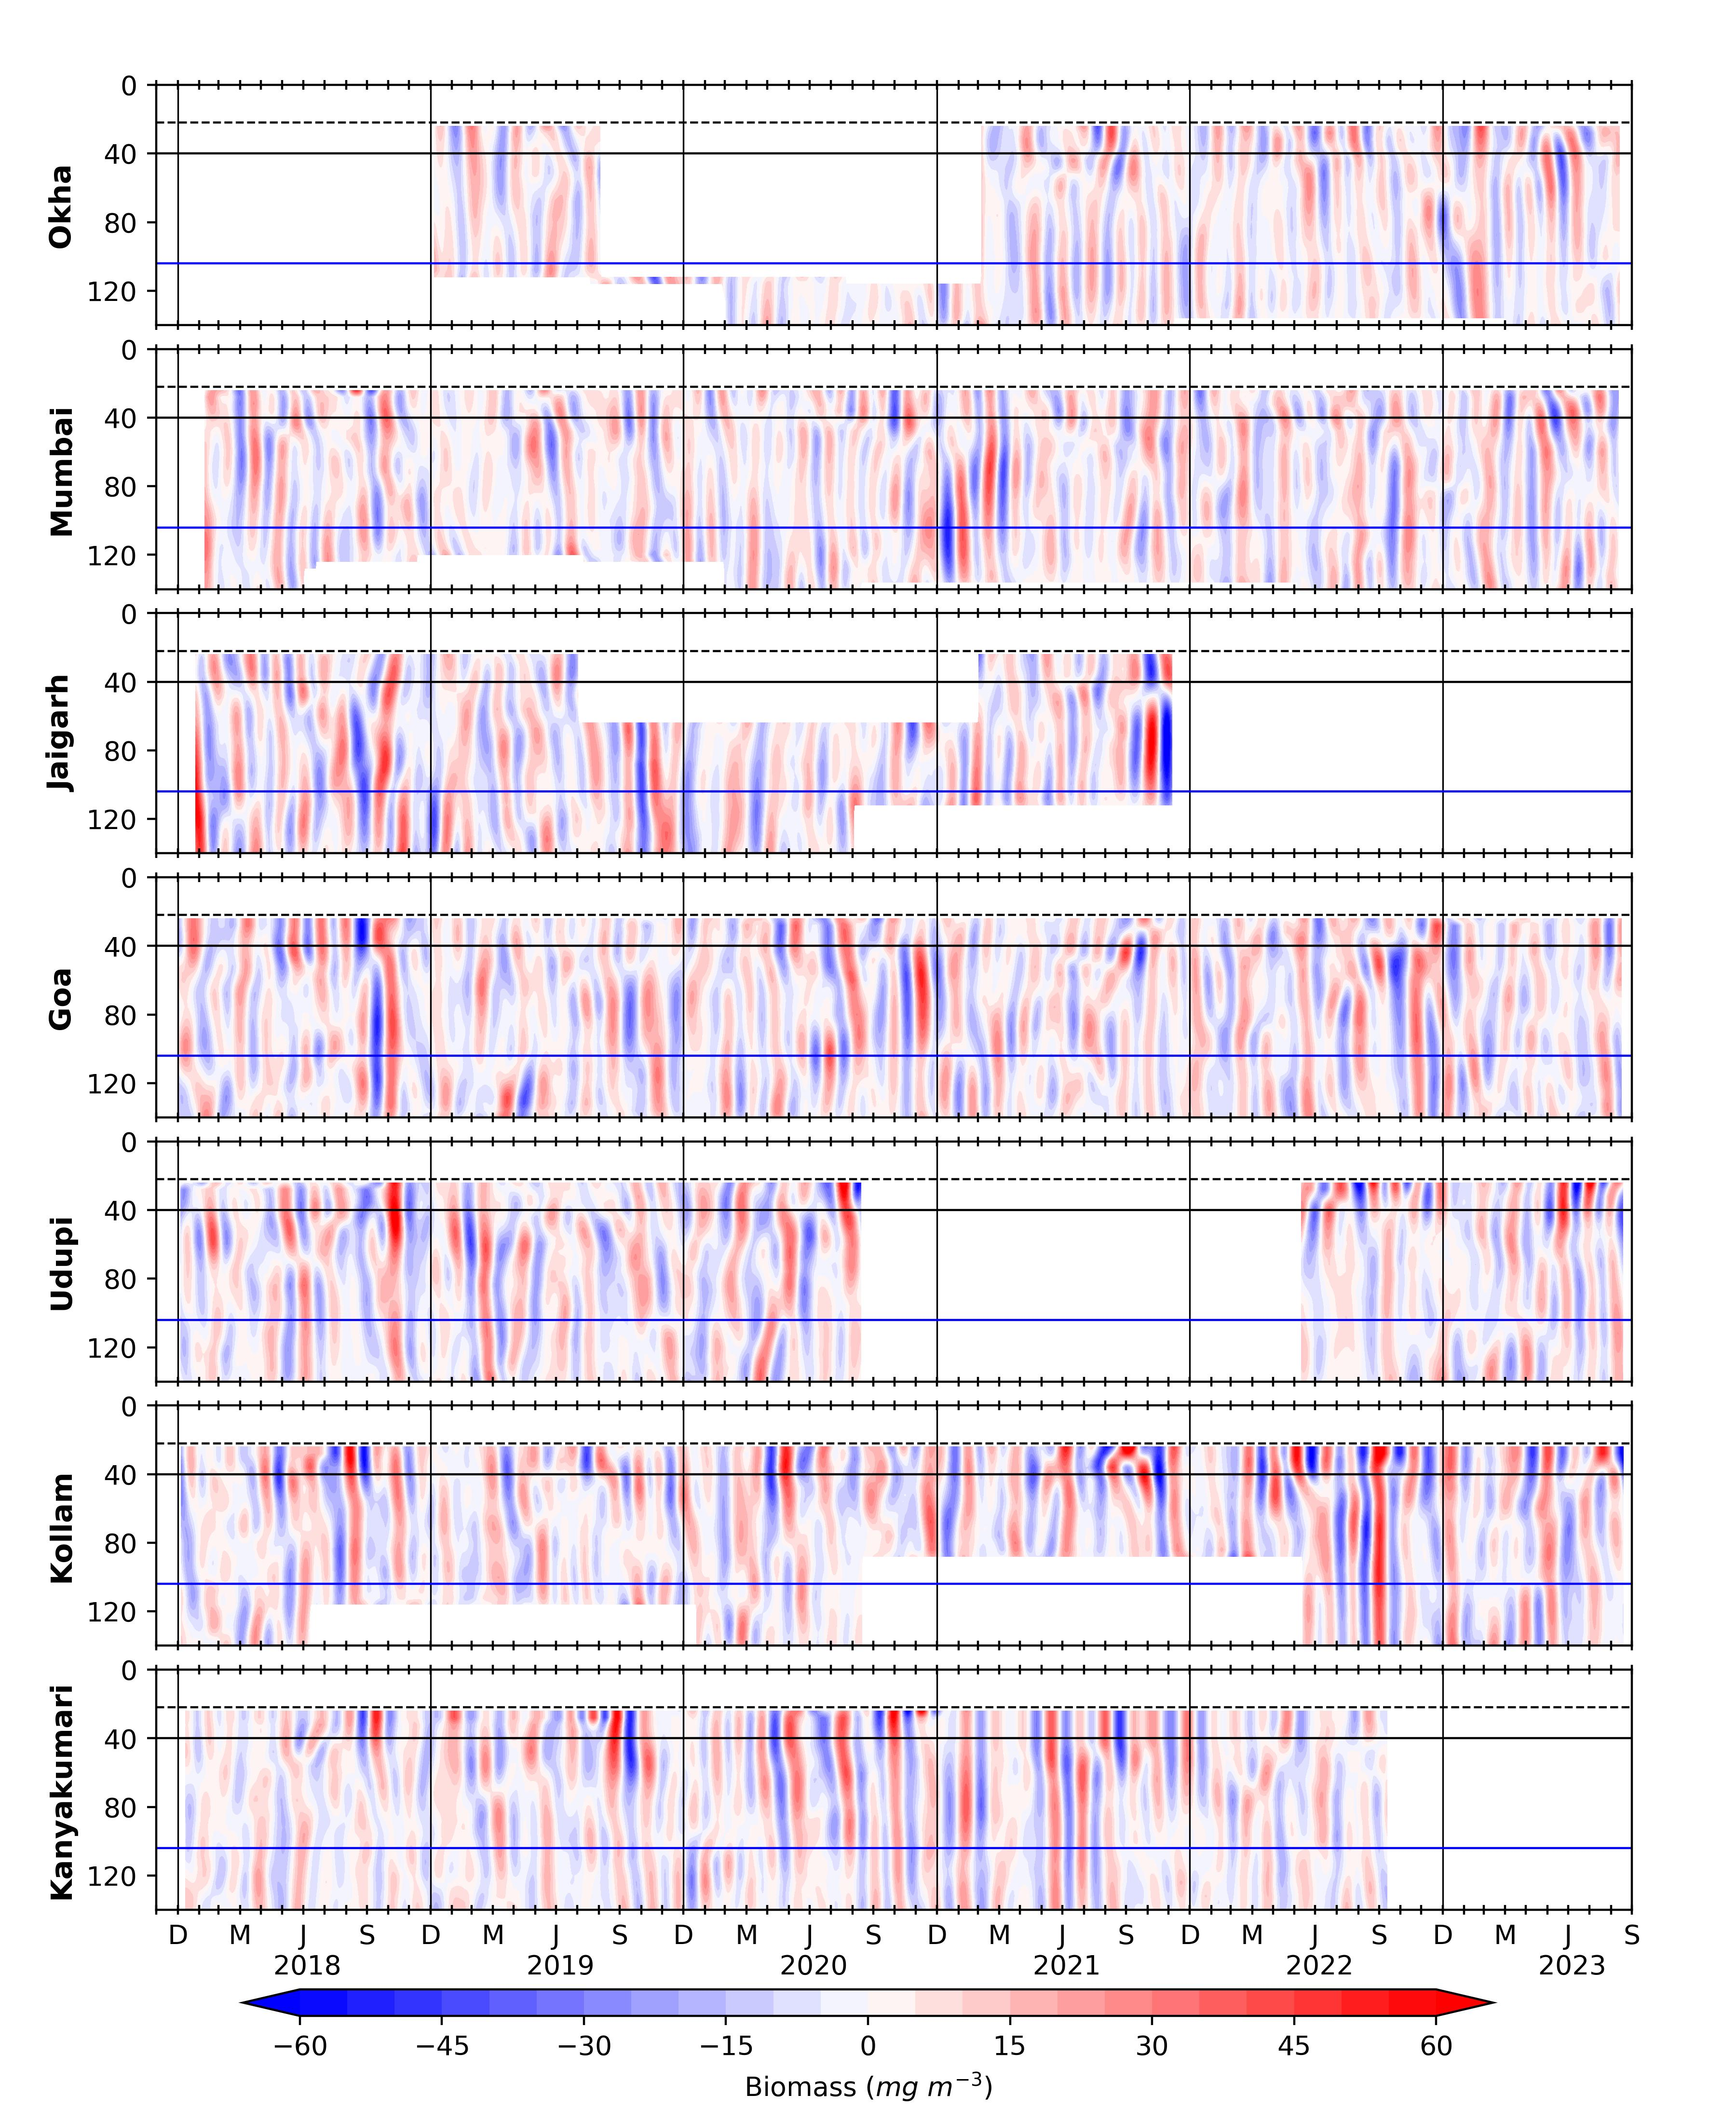
\includegraphics[width=\textwidth]{/media/scilab/disk_ranjan/works/backscatter_wc/figures/intraseasonal_30_90_181.jpeg} 
	\captionsetup{justification=justified,font=footnotesize,skip=0.05\baselineskip,width=\textwidth}
	\caption{Biomass variation found in the Intraseasonal band i.e., 30 to 90 days  period is obtained using a lanczos band pass filter. The horizontal black and blue lines is for 40 and 104 m;
	%, and the standard deviation of biomass at those depths are shown in respective colors at top right corner of each panel
	vertical black lines separate the years and solid magenta curves denotes D215 (D175 off Okha and Kanyakumari). The dashed line at 22 m marks the top-depth of first bin i.e, 24 m. Intraseasonal variability is seen throughout the record, is coherent along the slope and its magnitude is stronger during August to November.}
	\label{fig:intraseasonal}
\end{figure}


\begin{figure}[htbp]
	\centering
	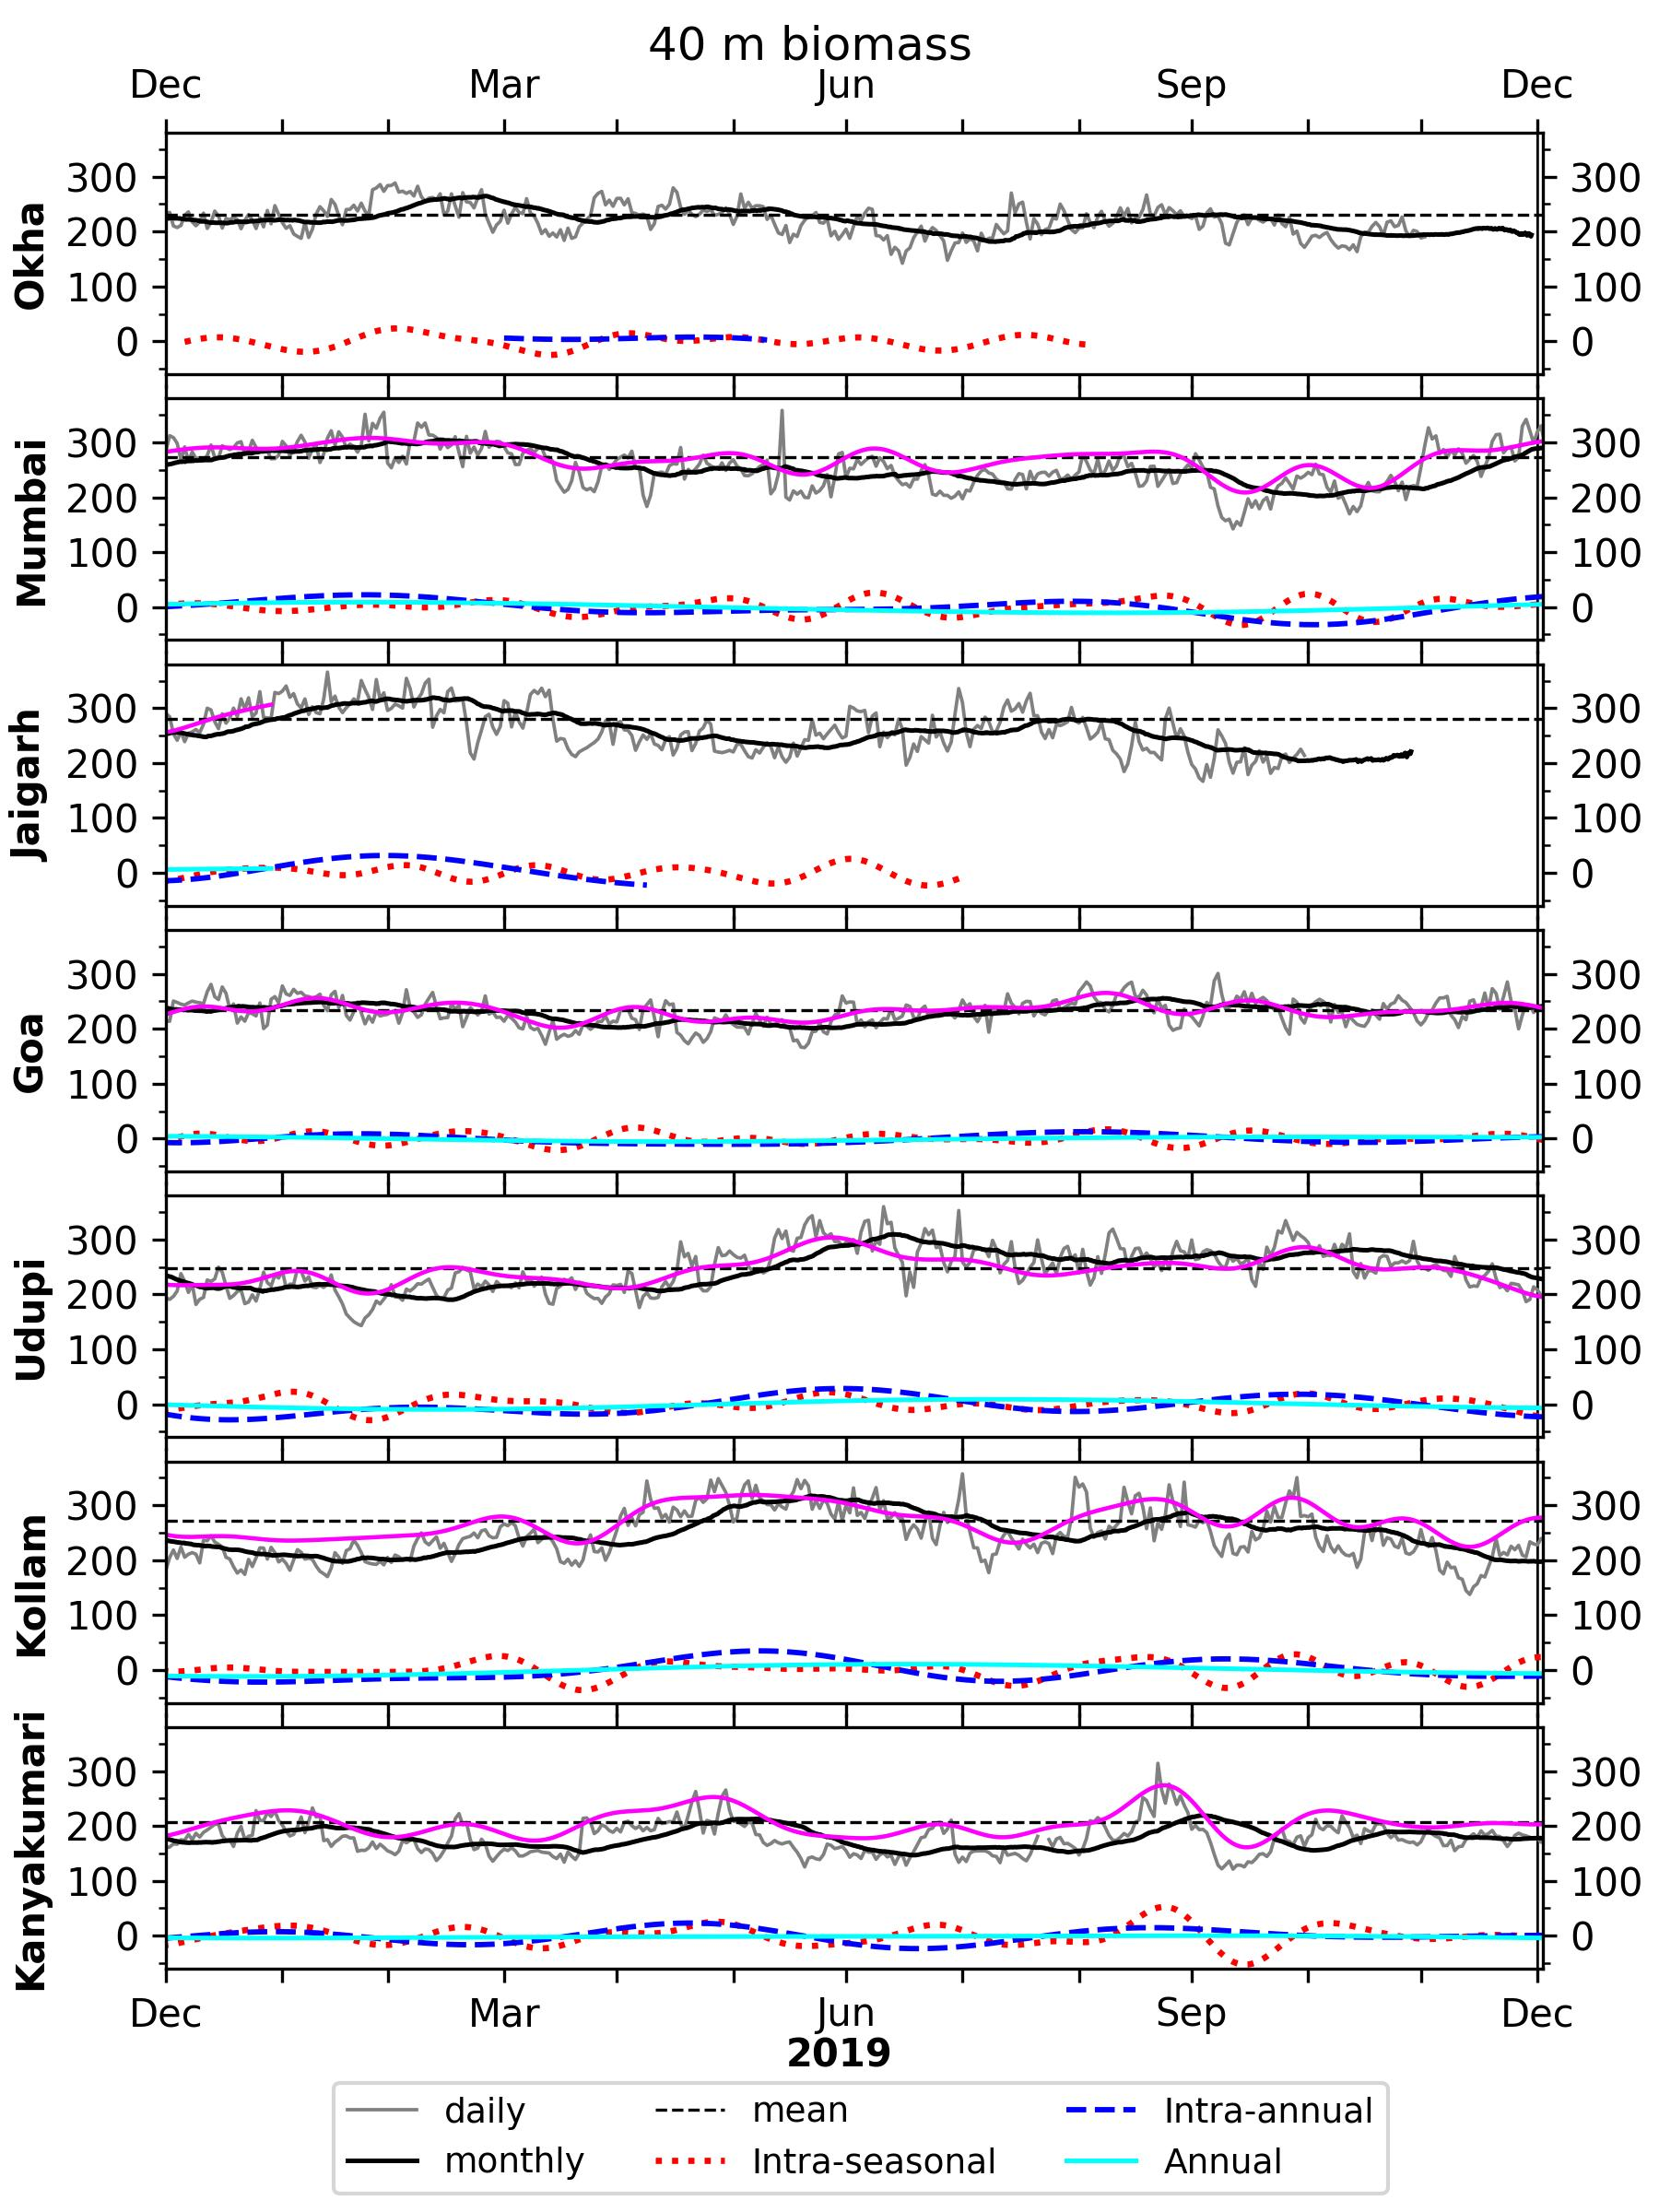
\includegraphics[width=\textwidth]{/media/scilab/disk_ranjan/works/backscatter_wc/figures/biomass_40m_2019.jpeg} 
	\captionsetup{justification=justified,font=footnotesize,skip=0.05\baselineskip,width=\textwidth}
	\caption{Comparison between mean-removed daily biomass time series at 40 m and the distinct components of variability off Mumbai, Goa and Kollam for 2019. The biomass units are mg~m$^{-3}$ and its mean for respective location is shown in top right box. Off Mumbai and Kollam, an increase in biomass is noticed from May onward and lasting till late monsoon with weeks of low biomass during August due to low contribution of intraseasonal component of variability. The pink (green) highlighted region shows coherence in 30--90 days intraseasonal band (daily data) of 40~m biomass. The standalone spikes are representative of patchiness i.e., dense clusters of zooplankton and may not necessarily be observed elsewhere. The annual variability is very weak and lies close to zero almost always.}
	\label{fig:variability}
\end{figure}



\end{document}
